% Template Credit to:
% A. Thall, 2003
% R. Roos, 2013
% G. Kapfhammer, 2017
% OBC, 2018

\documentclass[12pt]{report}


% use varepsilon
\DeclareSymbolFont{epsilon}{OML}{ntxmi}{m}{it}
\DeclareMathSymbol{\epsilon}{\mathord}{epsilon}{"0F}

\topmargin -4em
\setlength{\textwidth} {420pt}
\setlength{\textheight} {620pt}
\setlength{\oddsidemargin} {20pt}
\setlength{\marginparwidth} {72in}

\usepackage[bottom,single]{gatorthesis} % for final department copy
% \usepackage[debug,draft,single]{gatorthesis} % for student workcopy
%\usepackage[single]{gatorthesis} % for student
%\usepackage[debug,draft,nolists,nofront,single]{gatorthesis} % more options

\usepackage{comment}
\usepackage{amsmath}
\usepackage{amssymb}
\usepackage{url}
\usepackage{graphicx}

% custom packages
\usepackage{fancyhdr}
\usepackage{hyperref}
\usepackage{subcaption}
\usepackage{mathtools}
\usepackage[utf8]{inputenc}
\usepackage[T1]{fontenc}
\usepackage{mathptmx}
\usepackage{listings}
\usepackage{mdframed}
\usepackage{tikz}

\usetikzlibrary{arrows, positioning}

% may not work with travis ci
\usepackage{color}

% Use elastic spacing around the headers
\usepackage{titlesec}

\lstset{
  columns=fixed,
  keywordstyle=\color{black}\bfseries, % bold black keywords
  basicstyle=\small, % print whole listing small
  identifierstyle=, % nothing happens
  commentstyle=\color{white}, % white comments
  stringstyle=\ttfamily,
  showstringspaces=false,
  basewidth=0.5em
}

% set it so that subsubsections have numbers and they
% are displayed in the TOC (maybe hard to read, might want to disable)
\setcounter{secnumdepth}{3}
\setcounter{tocdepth}{3}

\setlength{\parindent}{0pt}
\setlength{\parskip}{0.1in}

% this should give you the ability to use some math symbols that
% were available by default in standard latex (i.e. \Box)
\usepackage{latexsym}

% define a little section heading that doesn't go with any number
% \newcommand\littlesection[1]{
%   \vskip 0.5cm
%   \noindent {\bf #1}
%   \vskip 0.0001cm
% }

\newcommand\todo[1]{
\begin{center}
  \color{red}
  {\bf TODO}\\
  #1
\end{center}
}

\newcommand\inlinetodo[1]{{\color{red} (TODO: #1)}}

% custom commands
\newcommand{\name}{{\sc RayTerm}}
\newcommand{\rayorg}{\vec{R_{origin}}}
\newcommand{\raydir}{\vec{R_{direction}}}

\begin{document}

\thesistitle{{\large \name:}\\{A Ray-Tracing Rendering Engine for XTerm-like Terminals}}

\thesisauthor{Saejin Mahlau-Heinert} \thesisadvisor{Dr. Janyl Jumadinova}

\thesisnumber{CS-2019-10}

\thesisreadera{Dr. Gregory Kapfhammer}

\date{\FileRevised \\ $\mbox{}$Revision: 1.8 $\mbox{}$}

\thesismaketitle
\thesismakecopyright

%   ********************************************************************
%   * YOU MAY SPLIT YOUR THESIS INTO SEVERAL FILES AND "\include" THEM *
%   * AS SHOWN BELOW. FOR INSTANCE, FILE "abstract.tex" CONTAINS THE   *
%   * ABSTRACT, FILE "ack.tex" CONTAINS THE ACKNOWLEDGMENTS, ETC. YOU  *
%   * MAY, OF COURSE, PUT EVERYTHING INTO ONE HUGE FILE, BUT THERE ARE *
%   * ADVANTAGES TO SPLITTING THINGS UP--FOR EXAMPLE, YOU CAN COMMENT  *
%   * OUT "\include" LINES OF SOME PARTS IN ORDER TO PRINT DRAFTS      *
%   * CONTAINING SELECTED SECTIONS OF YOUR THESIS, SAVING PAPER AND    *
%   * PRINTING COSTS.                                                  *
%   *                                                                  *
%   * YOU ARE NOT REQUIRED TO HAVE A "dedication"--IF YOU DON'T, JUST  *
%   * DELETE THAT LINE OR COMMENT IT OUT WITH A LEADING "%"            *
%   ********************************************************************

\begin{abstract}
  Over the many years of innovation in the field of computer graphics, advances in rendering have led to massive increases in the fidelity of engaging, satisfying, and realistic computer visualizations.
  \name\ is a new and unique entry into the ranks of rendering engines, and makes its own contributions to the field of computer graphics.
  While harkening back to the retro aesthetics of the seventies and eighties, \name\ embraces new advances in computing power to bring fully ray-traced visuals to an old screen -- the terminal.
  Using Unicode block characters to simulate pixels and a ray-tracer written in C++, \name\ will render a fully three-dimensional (3D) scene, complete with lighting, shadows, and physically-based materials.
  \name\ can be used as an engine for terminal-based 3D tools, visualizations, games, and more; it will be fully open-source and ready for integration into other projects.

\end{abstract}
  % REQUIRED!

% \include{dedication} % OPTIONAL

% \include{ack}       % OPTIONAL, BUT ALMOST EVERYONE INCLUDES IT

%   ********************************************************************
%   * FRONT MATTER--TABLE OF CONTENTS, ETC. YOU PROBABLY DON'T NEED TO *
%   * CHANGE ANY OF THIS UNLESS YOU HAVE NO TABLES OR FIGURES, OR YOU  *
%   * WANT TO CHANGE NUMBERING DEPTH FOR SUBSECTIONS, OR ...           *
%   ********************************************************************

\tableofcontents
%\listoftables       % OMIT THIS IF YOU DON'T HAVE ANY TABLES
\listoffigures      % OMIT THIS IF YOU DON'T HAVE ANY FIGURES

%   ********************************************************************
%   * A GLOSSARY IS ALMOST NEVER NEEDED UNLESS YOU HAVE AN UNUSUALLY   *
%   * LARGE NUMBER OF SPECIAL TERMS OR NOTATIONS AND IT WOULD DETRACT  *
%   * TOO MUCH FROM THE FLOW OF THE PAPER TO DEFINE THEM IN-LINE.      *
%   ********************************************************************
%\include{glossary}  % OMIT THIS IF YOU DON'T HAVE A GLOSSARY (FEW PEOPLE DO)

% ch:intro
%
% $Id: ch01_overview
%
%   *******************************************************************
%   * SEE THE MAIN FILE "AllegThesis.tex" FOR MORE INFORMATION.       *
%   *******************************************************************

\chapter{Introduction}
\label{ch:intro}

In the early days of computing, real-time rendering engines that powered games like {\it Doom} or {\it NetHack} had to run on extremely underpowered hardware and render on low-resolution screens.
The dream of real-time, photorealistic graphics was far, far away.
However, even then the simple, blocky graphics, easily recognizable shapes, and maze-like environments were fantastic entertainment.
Today the retro-style of low-resolution graphics, pixel art, and 8-bit color is abound in the gaming space.
\name\ is one part of enabling that retro-aesthetic to grow into a new and unique style that, while similar to the old classics, can be more engaging and real than they ever were.

This thesis document describes a system that creates a moving image on a terminal screen.
The system is called \name; it performs real-time updating of the displayed image, generating a window into a three-dimensional world, applicable for a wide variety of programs.
With the current generation of powerful CPU and GPU chips, able to execute billions and trillions of calculations per second respectively, it is finally possible to do real-time, close to photorealistic rendering.
While the goal of \name\ is not high-resolution photorealism, some approximation of photorealism will be obtained, albeit at a lower resolution.

\section{Motivation} \label{ch:intro:motivation}

\section{Overview}
\label{ch:intro:overview}

\name\ uses the recursive ray-tracing algorithm, simulating the path of light through the scene -- this is described in more detail in Section~\ref{ch:intro:overview:raytracing}.
Rendered images are displayed in two different modes; the first uses single half-character pixels, and the second more complex Unicode block characters.
The mechanics of this image composition method are discussed in Section~\ref{ch:intro:overview:unicode}.
Once an image is rendered, the \texttt{ncurses} C library \cite{ncursesLibrary} is used to display it in a terminal.
An example of the final terminal output is Figure~\ref{fig:checker_metal}, which was generated by TerminalImageViewer \cite{tivGithub} as a mockup \inlinetodo{this should be an actual output image, and described as such}.
More details on this process are given in Section~\ref{ch:intro:overview:ncurses}.

\begin{figure}[htb]
  \centering
  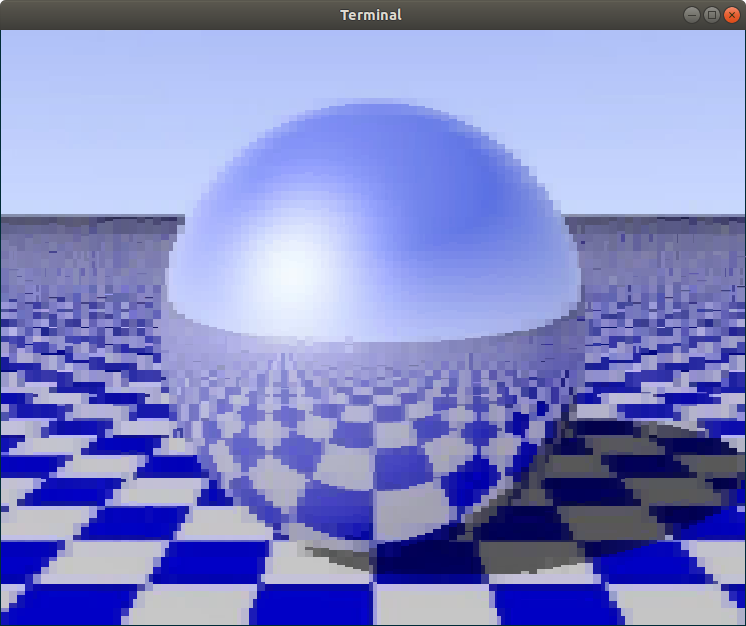
\includegraphics[width=0.8\textwidth]{resources/checker_metal}
  \caption{Example of proposed terminal output}
  \label{fig:checker_metal}
\end{figure}

\subsection{Rendering Engines and Ray-Tracing}
\label{ch:intro:overview:raytracing}

A rendering engine is an algorithm that takes a scene -- a description of some collection of objects -- and generates an image or visual representation of that scene.
There are many different algorithms that accomplish this goal.
In this proposal, the recursive ray-tracing algorithm first pioneered by Turner Whitted in his ground-breaking paper {\it An Improved Illumination Model for Shaded Display} \cite{whitted1980improved}, will be discussed and utilized.
Ray-tracing was one of the first algorithms developed in the field of computer graphics, and although there have been some improvements since then, the idea behind the algorithm has maintained its original simplicity.

Ray-tracing has been used as the renderer of choice for photorealistic images, because with only a few modifications to Whitted's original algorithm, it can generate fantastic images.
In the past, however, render times have been so slow that it was impossible to generate images fast enough for real-time use.
For example, Figure~\ref{fig:povray_render} is a render created by the POV-Ray engine \cite{povray}.
POV-Ray can take between a few minutes to several hours to complete one single image depending on the processing power involved.
However, there have been a few recent innovations that change this, such as NVIDIA's RTX hardware acceleration.
Section~\ref{ch:intro:background:hardware} provides more details on these advances, as well as an explanation of how ray-tracing will be utilized in \name.

\begin{figure}[htb]
  \centering
  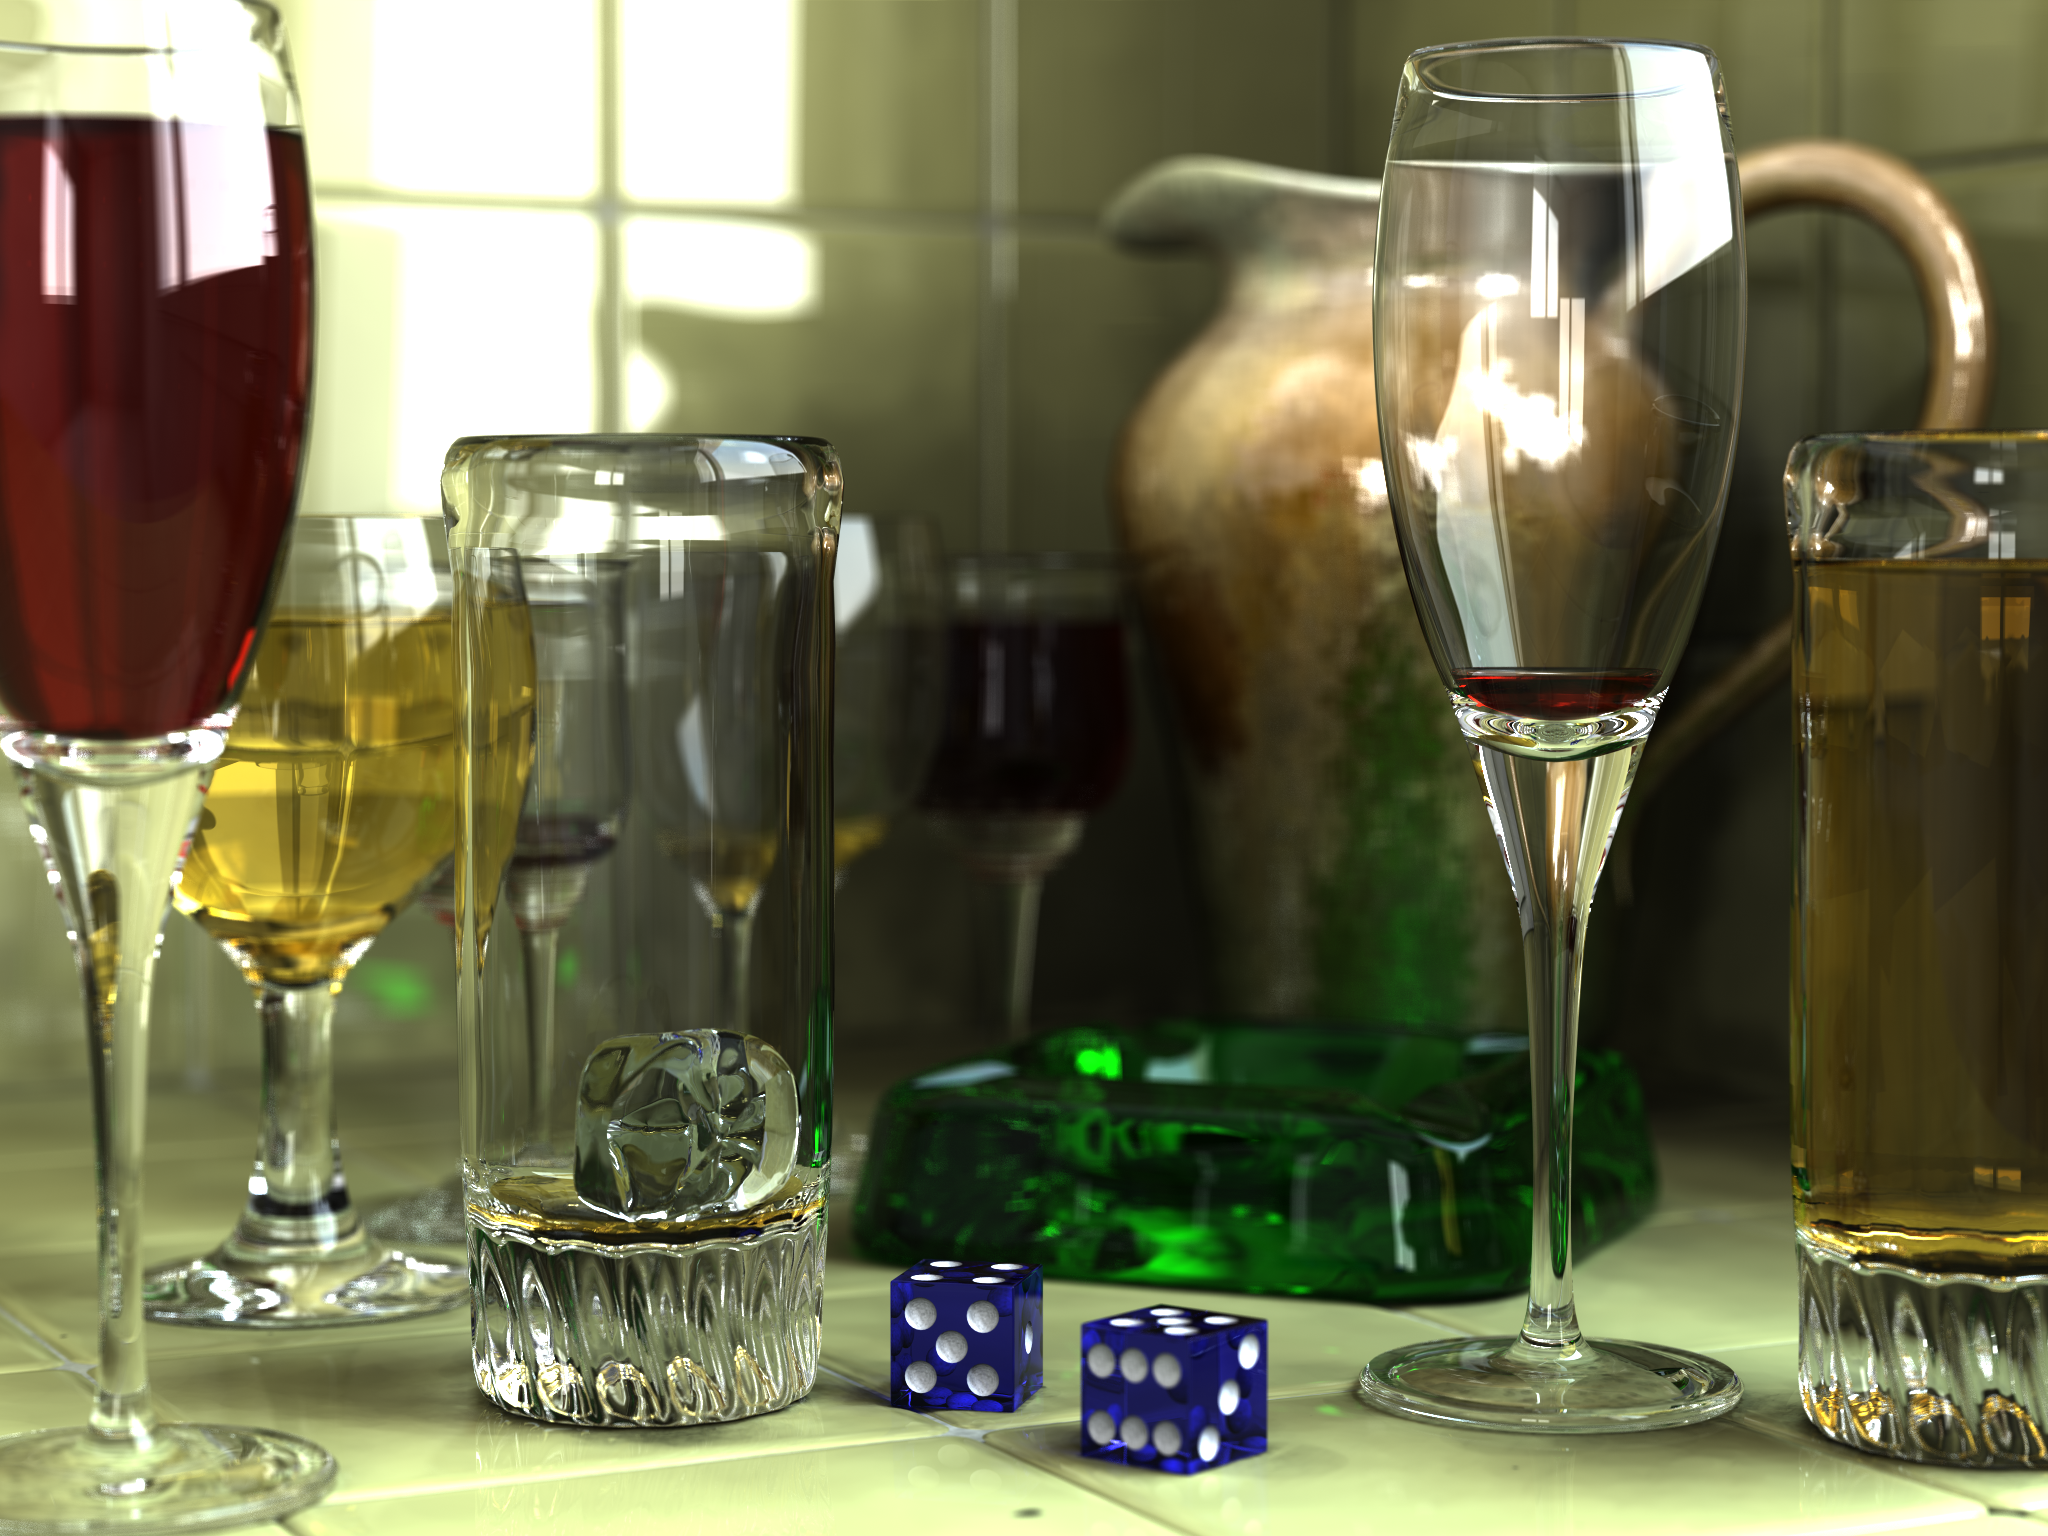
\includegraphics[width=0.8\textwidth]{resources/glasses_povray}
  \caption{POV-Ray render created by Gilles Tran \cite{povray2006render}}
  \label{fig:povray_render}
\end{figure}


Ray-tracing revolves around the idea of {\it rays}, a mathematical construct which can be defined by two vectors: an origin point, referred to as $\rayorg$ for some ray $R$, and a direction, referenced as $\raydir$.
These two vectors together represent a ray of infinite length that starts at the origin and projects along the direction.
An important addition to the concept of rays is a point along a ray -- this can be defined by using a third variable, $t$, to represent how far along the ray the point is located.
Therefore, Formula~\ref{equation:point_on_ray} can be used to get the coordinates of a point in three-dimensional space (assuming $\raydir$ is a unit vector).
This is called the {\it parametric~form} of a ray.
The mathematics behind ray-tracing are further explored in Section~\ref{ch:intro:background}.

\begin{equation}
  \label{equation:point_on_ray}
  \vec{point} = \rayorg + t\raydir
\end{equation}

In ray-tracing, rays are used to simulate the path that light takes as it travels around the scene.
When a ray intersects with an object in the scene various interactions take place that simulate how light may travel under different conditions.
It is worth noting that a base assumption is made in ray-tracing when using straight rays as described here: light follows a straight line without changes.
This is only the case in reality when light travels through a vacuum with no gravitational bodies; thus, basic ray-tracing is not exactly photorealistic and does not model phenomena like atmospheric scattering.
Additional mathematics and systems must be used to bend, attenuate, or scatter a ray to accurately render transparent volumes -- this is called volumetric ray-tracing.
Volumetric ray-tracing will not be supported by the proposed \name, but would be a fascinating area of future work.

The basis for ray-tracing is the rendering equation, articulated by James Kajiya in 1986 \cite{kajiya1986rendering}.
The rendering equation models the outgoing light at some point given all incoming light, a bidirectional reflectance distribution function (BDRF), and a normal for the surface at the point modeled.
If solved for every point in the scene, the rendering equation could generate a completely photorealistic image -- this would, however, require massive amounts of computation.
This is because the rendering equation contains an integral over all incoming light which must be solved through numerical analysis.
Ray-tracing engines that do this are known as {\it path-tracers} and are the most photorealistic rendering engines invented.

\name\ will not use a path-tracer -- such algorithms are still many times too slow for most real-time rendering situations.
Instead, the rendering equation will be solved by sampling the incoming light with rays.
This is known as recursive ray-tracing, since it starts with a single ray that splits every time it encounters a surface.
The eventual goal of the recursive ray-tracing algorithm is to create a tree of rays for each {\it fragment} to render.
A fragment is either a pixel or some sub-pixel -- many systems will use four or more fragments per pixel to get better anti-aliasing and more accurate results.
Each ray contains some color that represents the color of the light in that ray.
When a ray hits an object, it is {\it scattered} by the {\it material} of the object, splitting and generating new rays.
These rays are biased towards directions that contain lots of incoming light -- such as towards a point light source.
The specific implementation of recursive ray-tracing that \name\ will use will only scatter into a set number of rays at each intersection point: one ray toward each light source, along with reflection and refraction rays towards the relevant directions.

The base of each generated tree is an {\it eye-ray} -- a ray with its origin at the fragment location on the camera plane.
The eye-ray's color is the color that will be rendered for that fragment.
As the eye-ray projects forward, away from the eye, it is tested for intersection with all objects in the scene.
When an intersection happens and the generated rays scattered, the eventual color values of the scattered rays are combined to produce the color of the original eye-ray.
This is done recursively to fully render the scene.


\subsection{Image Composition using Unicode Characters}
\label{ch:intro:overview:unicode}

Unicode is a character standard that allows anyone to reference many thousands of characters to compose text, no matter the environment around the text \cite{unicode}.
Some critical characters that \name\ will use are known as the {\it block characters} -- they are characters \texttt{U+2580} -- \texttt{U+259F}.
Relevant characters are shown in Figure~\ref{fig:unicode_characters}.
Contingent on the quality of the output using only block characters, additional sets could be used, such as triangles and lines.
The core of image composition using Unicode is an algorithm coloring the characters and the background -- \name\ will use this algorithm on every character of the output to both determine the character to display, and the foreground and background colors for that character.
The foreground colors the character itself, whereas the background provides a relief color.
This allows each {\it character~pixel} to represent a hard gradient.

\begin{figure}[htb]
  \centering
  \hspace{0.3em}
  \begin{subfigure}[htb]{0.4\textwidth}
    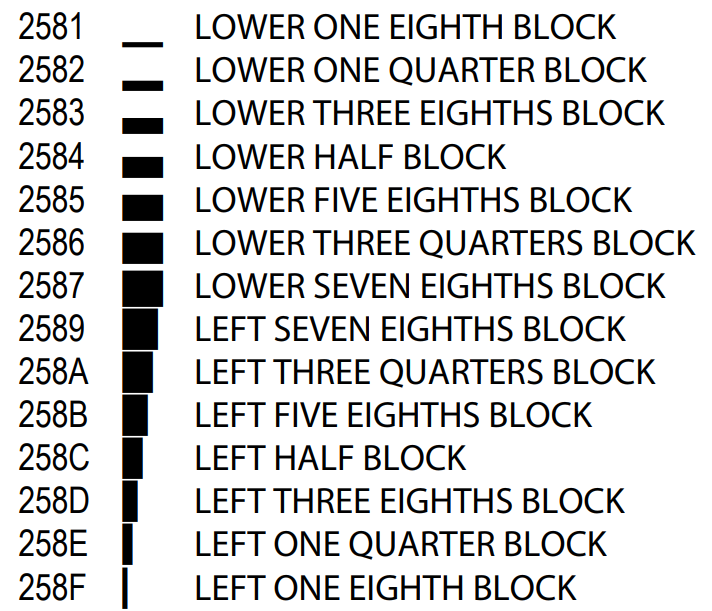
\includegraphics[width=\textwidth]{resources/block_elements}
    \caption{Block Elements}
    \label{fig:unicode_block_characters}
  \end{subfigure}
  \hfill
  \begin{subfigure}[htb]{0.51\textwidth}
    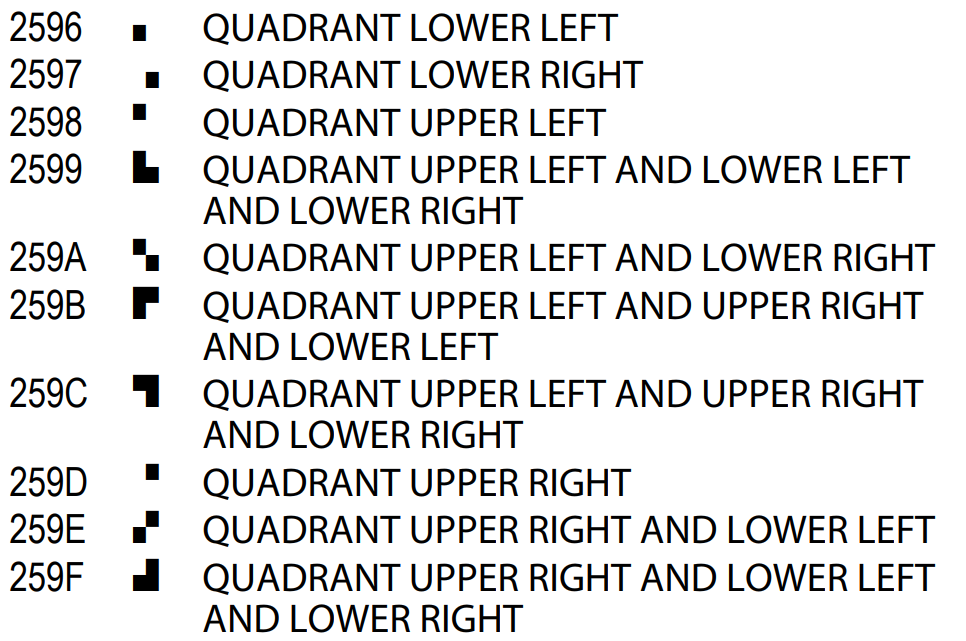
\includegraphics[width=\textwidth]{resources/quadrant_elements}
    \caption{Quadrant Elements}
    \label{fig:unicode_quadrant_characters}
  \end{subfigure}
  \caption{Subset of \texttt{U+2580} -- \texttt{U+259F} \cite{unicode}}
  \label{fig:unicode_characters}
\end{figure}

There are two image modes that will be available for use in \name.
The first is pure {\it pixel mode}, in which the Unicode ``half-block'' symbol (\texttt{U+2584}) is used.
Since mono-spaced character output (such as in a terminal) is twice as tall as it is wide, the half-block can split a single character into two pixels that are colored differently: the upper pixel with the background color of the character, and the lower with the character or foreground color of the pixel.
This would mean that a typical 85 by 30 character terminal would result in a screen space of 85 by 60 pixels.
This mode also dramatically reduces the number of ray-tracing computations needed, since only one ray per pixel is required.

The second image mode is considerably more complicated and slower, as it uses significantly more rays per character in order to determine what Unicode block character most fits the desired output.
On the other hand, it allows a much higher perceived resolution, since the characters used have smaller footprints of down to an eigth of a character in width or length.
The differences between these two modes are highlighted in Figure~\ref{fig:unicode_mode_comparison1} and~\ref{fig:unicode_mode_comparison2}.
It can be seen that the first image mode, {\it pixel mode}, shows a rather fuzzy definition of the main large sphere.
However, in the second image mode, {\it character mode}, the sphere and the reflections seen in it are much more defined.
The performance impact of both modes is another factor that must be assessed when making implementation decisions for \name.

\begin{figure}[htb]
  \centering
  \begin{subfigure}[htb]{0.49\textwidth}
    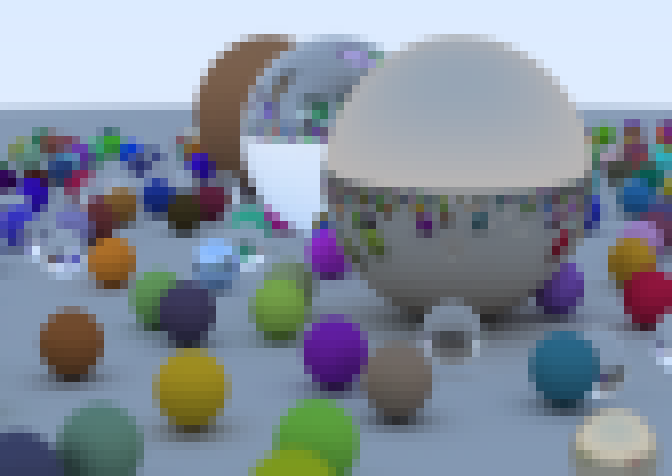
\includegraphics[width=\textwidth]{resources/many_spheres_square}
    \caption{Pixel Mode Image Output}
    \label{fig:unicode_mode_comparison1}
  \end{subfigure}
  \hfill
  \begin{subfigure}[htb]{0.49\textwidth}
    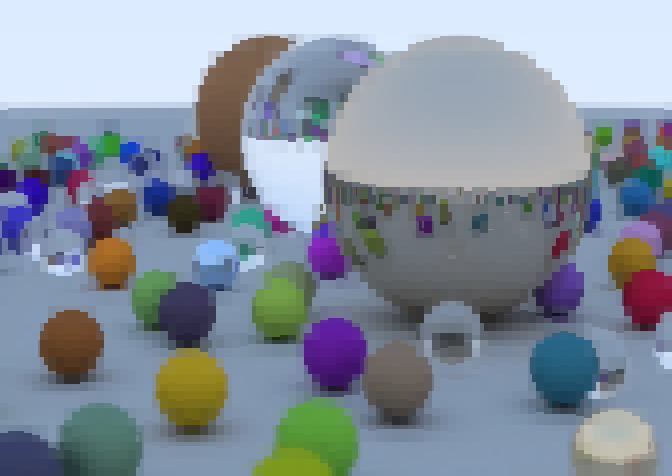
\includegraphics[width=\textwidth]{resources/many_spheres}
    \caption{Character Mode Image Output}
    \label{fig:unicode_mode_comparison2}
  \end{subfigure}
  \caption{Examples of Image Mode Output}
  \label{fig:unicode_mode_comparison}
\end{figure}

\subsection{Terminal Output using \texttt{ncurses}}
\label{ch:intro:overview:ncurses}

Once an image is generated, \name\ must somehow display that image in a terminal with no surrounding prompt or other formatting -- just a simple {\it character field}.
To do this, we will use \texttt{ncurses}, a C library that abstracts implementation details of the terminal to enable full-window 24-bit color character output.
Using \texttt{ncurses}, the terminal window will be divided into two ``panels'', a main panel for the actual image output -- updated 30 to 60 times per second -- and an info panel to render information such as frames per second and logging information.
With this dependency, \name\ can be used on all terminals that support \texttt{ncurses} -- generally, any XTerm-like terminal will work, as long as it supports a terminal information database: either \texttt{termcap} or \texttt{terminfo} will work.

A possible limitation to \texttt{ncurses} is keyboard input handling -- there is no mechanism to get events on an up or down movement of a key, as is possible in some other libraries.
Therefore, research will need to be done on possible alternatives for the input aspect of the engine.
This is not a priority, however, since it is not related to the rendering nature of \name and instead only helps with demonstrations of its capabilities.


\section{Background} \label{ch:intro:background}

The background information for the algorithms and techniques used to implement \name\ are discussed in this section.
We introduce basic vector mathematics in Section~\ref{ch:intro:background:vector_math}.
In Section~\ref{ch:intro:background:raytracing_math} we detail most of the mathematics involved.
In \name, many of these algorithms are implemented behind the scene in APIs like OptiX and CUDA \inlinetodo{update with actual implementation location}.

\subsection{Vector Mathematics}
\label{ch:intro:background:vector_math}


\subsection{Raytracing Mathematics}
\label{ch:intro:background:raytracing_math}
The mathematical basis for ray-tracing is heavily dependent on understanding vector mathematics -- Section~\ref{ch:intro:background:vector_math} is a small introduction to such mathematics.
The algorithms described below are run millions of times per second in a highly parallelized environment.
In this context, parallelization is a technique for running two or more algorithms simultaneously; therefore even minor optimizations are extremely important since they reduce the overall time to render.
All of the ray-tracing mathematics described here are synthesized from Peter Shirley's excellent {\it Ray Tracing in One Weekend} \cite{shirley2016ray} and the Morgan Kaufmann textbook {\it Physically Based Rendering: From Theory to Implementation} \cite{pharr2016physically}.

Scenes that can be ray-traced must be a collection of surfaces that are mathematically intersectable with a ray.
Any surface that can be defined by a implicit surface definition function, in the form of Function~\ref{equation:surface_equation}, is intersectable with a ray \cite{pharr2016physically}.
In Function~\ref{equation:surface_equation} and for the rest of this section, $\vec{p}$ is a vector representing a point in three-dimensional space.
The implicit surface definition function must have the property that if and only if $f(\vec{p})$ is $0$, then $\vec{p}$ is on the defined surface.
The point of intersection between a ray and a surface defined in this way can be found by solving Equation~\ref{equation:ray_surface_intersection} for $t$ and then using Formula~\ref{equation:point_on_ray} to calculate the coordinates of that point on the ray.

\begin{equation}
  \label{equation:surface_equation}
  f(\vec{p}) = 0
\end{equation}

\begin{equation}
  \label{equation:ray_surface_intersection}
  f(\rayorg + t\raydir) = 0
\end{equation}

In \name, the only surfaces that are supported are spheres, triangles, and infinite planes, since their surface definition functions are mathematically simple.
If there is additional development time and resources available, other shapes such as quads, arbitrary polygons, and cubes may be considered.
This may not be a huge development effort, as the algorithm discussed for triangle intersection testing is applicable to any convex polygon.
A sphere is the simplest three-dimensional object to calculate ray intersection with, and therefore will be the first implemented for \name.
In fact, during feasibility testing much of the math described in this section was implemented in the Go programming language.

\littlesection{Ray-Sphere Intersection}

The surface definition function of a sphere is Function~\ref{equation:sphere_surface}, with $S$ representing the sphere.
The intersection point between a ray and a sphere is given by solving Equation~\ref{equation:ray_sphere_intersection} for $t$ and then using Formula~\ref{equation:point_on_ray}.
Both of these equations are directly adapted from {\it Ray Tracing in One Weekend} \cite{shirley2016ray}.
Notice that Equation~\ref{equation:ray_sphere_intersection} is quadratic, and the number (and values) of the roots give us the $t$ we want to use.
The smallest positive root corresponds to the point on the ray which first intersects the sphere.
If there are no real roots, then the ray does not intersect the sphere.

\begin{equation}
  \label{equation:sphere_surface}
  f(\vec{p}) = (\vec{p} - \vec{S_{center}})^2 - {S_{radius}}^2
\end{equation}

\begin{equation}
  \label{equation:ray_sphere_intersection}
  (\raydir^2)t^2 + 2(\raydir \cdot (\rayorg - \vec{S_{center}}))t + (\rayorg - \vec{S_{center}})^2 - {S_{radius}}^2 = 0
\end{equation}

\littlesection{Ray-Plane Intersection}

For any two-dimensional object, the plane it lies in is the first shape tested for intersection.
Luckily, ray-plane intersection testing is fairly cheap and straight forward.
The surface definition function of a plane is Function~\ref{equation:plane_surface}, with $P$ representing the plane.
The plane's {\it offset} is a point on the plane, and the plane's {\it normal} is a vector perpendicular to the plane.
The intersection point between a ray and a plane is given by solving Equation~\ref{equation:ray_plane_intersection} for $t$ and then using Formula~\ref{equation:point_on_ray}.
These equations were derived from basic vector math, along with guidance from {\it Physically Based Rendering} \cite{pharr2016physically}.

\begin{equation}
  \label{equation:plane_surface}
  f(\vec{p}) = (\vec{p} - \vec{P_{offset}}) \cdot \vec{P_{normal}}
\end{equation}

\begin{equation}
  \label{equation:ray_plane_intersection}
  (\vec{P_{normal}} \cdot \raydir)t + \vec{P_{normal}} \cdot (\rayorg - \vec{P_{offset}}) = 0
\end{equation}

\littlesection{Ray-Triangle Intersection}

The method for testing intersection with triangles is a bit more complicated than the other tests we've covered so far.
The mathematics for this section are again derived from vector mathematics.
However, Jean-Colas Prunier's {\it Scratchapixel}, an excellent and accessible online resource for 3D rendering \cite{prunier2017triangle}, was also an indispensable guide in facilitating understanding along the way.
First, intersection is tested with the plane the triangle lies in -- this results in a ray-plane intersection point $\vec{Q}$, or no intersection.
Then, if there was an intersection, another test must be performed to detect if $\vec{Q}$ is inside the triangle.
We do this using the ``inside-outside'' method (as suggested by {\it Scratchapixel}): test if $\vec{Q}$ is on the left side of each edge.

To conduct the left-side test, we label each triangle vertex $\vec{V_i}$, with $i$ increasing in the counter-clockwise direction.
We then have three triangle vertices: $\vec{V_0}$, $\vec{V_1}$, and $\vec{V_2}$.
We can now use Function~\ref{equation:left_edge_test}: if $f(i) > 0$ for each $i$, then $\vec{Q}$ is inside the triangle.
Otherwise, $\vec{Q}$ is outside the triangle.
Note that in Function~\ref{equation:left_edge_test}, if $i = 3$, then $i = 0$ ($i$ ``wraps'' to only valid values).

\begin{equation}
  \label{equation:left_edge_test}
  f(i) = P_{normal} \cdot ((\vec{V_{i+1}} - \vec{V_i}) \times (\vec{Q} - \vec{V_i}))
\end{equation}

Function~\ref{equation:left_edge_test} can be complicated to visualize, so imagine this: we first form two vectors, both with $\rayorg = \vec{V_i}$.
One points along the triangle's edge, while the other points to $\vec{Q}$.
Both of these vectors will be in the plane of the triangle.
Thus, if we cross them, the vector produced will either be away from the plane in the same direction as $\vec{P_{normal}}$, or away from the plane in the opposite direction.
According to the right hand rule, if the crossed vector is in the same direction as $\vec{P_{normal}}$, then the vector pointing to $\vec{Q}$ is ``to the left'' of the vector pointing towards $\vec{V_{i+1}}$.
We can then calculate the dot product between $\vec{P_{normal}}$ and the crossed vector -- if it is positive then the crossed vector is in the same direction as the normal, and therefore $\vec{Q}$ is to the left of the edge.
One last addendum to this intersection test is the fact that it can be difficult to perform the counter-clockwise numbering of vertices.
We will therefore simply expect vertices to be specified in counter-clockwise order.
This is similar to what many other 3D rendering programs assume.


\section{Development Ecosystem}
\label{ch:intro:background:development_ecosystem}

\name's development relied on many other systems -- the actual implementation code is hosted on Github, a public platform for projects using the Git version control system.
A continuous integration system called Travis CI \cite{travisci} was used for testing and environment management.
Documentation was handled by \texttt{doxygen} \cite{van2008doxygen} -- all external facing functions, methods, and classes have a minimum of a few sentences of documentation.
More details about the implementation tools are given in Section~\ref{ch:intro:background:languages_and_libraries}; testing hardware and low-level APIs are discussed in Section~\ref{ch:intro:background:hardware}.

\subsection{Programming Languages and Tools}
\label{ch:intro:background:languages_and_libraries}

With a large project such as \name, there are certain choices that must be made from a software development perspective.
These choices inform how the project is modified, built, and eventually executed.
In the case of \name, we used the C++ language \cite{cpp14standard} for main development, and Gradle \cite{gradle} as the build system.

\littlesection{Implementation Language}

The C++ language was used for three main reasons.
First, the language has a huge ecosystem of low-level tools, with interfaces to libraries such as OptiX, CUDA, FORTRAN-implemented mathematics like Blitz++, and much more.
This ensures that no matter the need, there was most likely a library out there that could fill that need.
Secondly, C++ allows low-level C-like programming while keeping abstractions such as objects available.
Lastly, C++ is a reasonably fast language: with no virtual machine, unlike Java or Kotlin, garbage collection is not a burden.
Decades of work have gone into compiler toolchains such as \texttt{g++} and \texttt{clang}, enabling optimizations that would not be possible for newer languages.

\name\ attempts to keep most of its implementation to a C-compatible level, using classes and greater abstractions only as necessary.
This ensures that overhead is minimal, as well as guaranteeing readability for the eventual open source release.
Advanced features of C++ such as templating are avoided so as to keep the knowledge entry barrier low.
Finally, all code in \name's implementation conforms to the Google C++ style guide \cite{googleStyleGuide}.

\littlesection{Build System}

Complex projects can be a nightmare to manage, especially when there are multiple contributors.
Build systems are an important tool that simplify this headache.
An opinionated build system such as Gradle also specifies sensible defaults for most situations, allowing minimal require configuration.
This is why Gradle was chosen as the build system for \name.
Gradle was used to compile C++ code into an executable for distribution or testing using its Software Model feature.
This feature allows the specification of executables and interdependent components, with sensible default source code and binary locations.
Gradle efficiently manages long linking or dependency lists, without resorting to macro-infested and variable-filled makefiles; it also handles header inclusions seamlessly, without dealing with relative path issues.
Gradle can even automatically retrieve dependencies if they are published as a Maven artifact.
All of these features make ongoing maintenance and development an easier proposition.

\subsection{Hardware}
\label{ch:intro:background:hardware}

There are many implementation issues related to the performance aspects of \name, since high performance is a strict requirement for obtaining render times low enough for real-time display.
For the purposes of testing, we used a machine with an Intel Core i7 4770k CPU and NVIDIA Geforce GTX 980Ti.
Only recently has ray-tracing even been able to achieve real-time levels of performance; much of this progress is thanks to advances in GPU technology.
The largest innovator in this space, GPU chip design company NVIDIA, released its RTX series of GPUs that have hardware support for ray-tracing.
RTX hardware spread is slow, however, due to its high early adoption cost.
Therefore we do not focus on RTX hardware; instead we look to slightly older technologies to provide the implementation backbone; this works well with the existing test hardware, which is a few generations old.

\todo{future section on what hardware API we actually use}
\todo{future section on how we delt with GPU vs CPU}

\section{Current State of the Art}\label{ch:intro:stateofart}

\section{Goals of the Project}\label{ch:intro:goals}
% This section could also be entitled ``Thesis'' or something similar.

% For an applied programming project, it is usually a statement about
% the feasibility and correctness of the approach used and the advantages it
%has over other approaches, using suitable metrics.

\section{Thesis Outline}\label{ch:intro:outline}
Chapter \ref{ch:relatedwork} reviews a number of past approaches
to the problem and summarizes their strengths and weaknesses. Chapter
\ref{ch:method} outlines the method of approach used to establish the
results.


% ch:relatedwork
%
% $Id: ch02_relatedwork
%
%   *******************************************************************
%   * SEE THE MAIN FILE "AllegThesis.tex" FOR MORE INFORMATION.       *
%   *******************************************************************
\chapter{Related Work}
\label{ch:relatedwork}

In this chapter, we will discuss a few related research papers, detail how they informed \name{}'s development, and show the improvements of \name{} over other systems.
First, we will conduct a high-level discussion of the first ray-tracing paper through to basic details on modern-day optimizations.
Following that, we will discuss two Github projects, one of which was a major inspiration for Unicode image composition and the algorithms involved (see Section~\ref{ch:intro:overview:unicode}).

\section{Discovery of Ray-Tracing}
\label{ch:relatedwork:discovery}

Here we describe the first ray-tracing paper, as well as two seminal works that brought ray-tracing to the forefront of photorealistic computer rendering.
It is important to note here that many of these papers are relatively old, since the algorithms being used in \name{} are correspondingly dated.
This is because most recent advances in ray-tracing concern more advanced methods of photorealistic rendering, such as path-tracing~\cite{lafortune1993bi}, low-level optimizations~\cite{wald2001interactive}, dynamic scene rendering~\cite{wald2007ray}, and volumetric ray-tracing hardware acceleration~\cite{kruger2003acceleration}, to name just a few.
All of these topics, while interesting and tangentially related, are too advanced; comparison with the algorithms used in \name{} would be unrealistic and meaningless, beyond showing how much more development \name{} needs to be truly state of the art when compared to modern ray-tracers.

\subsection{The First Ray-Tracer}
\label{ch:relatedwork:discovery:first}

The very first ray-tracing algorithm was developed by Arthur Appel in his 1968 paper ``Some techniques for shading machine renderings of solids''~\cite{appel1968some}.
His algorithm is now known as a ray casting algorithm\,---\,it does not follow the approach we described in Section~\ref{ch:intro:overview:raytracing}.
Instead, rays are traced from a point light source to the object being shaded, and a plus symbol of varying size is rendered at that location, depending on the intensity of light at that point.
When a photographic negative is taken, light spots that were not hit by the rays (thereby darkening them) are now ``in shadow'', as the color levels were inverted.
Today, Appel's work is not normally considered a real ray-tracing algorithm.
However, his work informed much of the following research, especially his ideas and mathematics on light intensity.
After Appel's work, there were some commercial applications of ray-tracing in the field of radiosity; ray-tracing was used to track radiation inside tanks at Mathematical Applications Group, Inc (MAGI)~\cite{whitted2018explains}.

\subsection{The Breakthrough}
\label{ch:relatedwork:discovery:breakthrough}

The next big entry to the ray-tracing field was Turner Whitted's 1980 paper ``An Improved Illumination Model for Shaded Display''~\cite{whitted1980improved}.
In this groundbreaking and approachable work, Whitted introduced the recursive ray-tracing algorithm we covered in Section~\ref{ch:intro:overview:raytracing}.
Whitted was not the first to use ray-tracing\,---\,Arthur Appel had first pioneered the field over a decade ago, and there were also emerging commercial applications.
Whitted's real contribution was the idea for how to improve ray-tracing so that it could solve the problem of {\it global illumination}.
Global illumination was not yet formalized, but the idea was to somehow gather the effect of all light in the scene on every single point.
This can easily be categorized as taking into account both direct lighting, light coming directly from a source, and indirect lighting, light coming from reflections, refractions, or other non-direct travel methods.

Recursive ray-tracing approximates direct lighting easily, as each encountered point sends a ray to each light in the scene.
Indirect lighting is slightly more difficult\,---\,pure reflection and refraction are easy, but as soon as reflections become more diffuse, and there are many, many directions a point gets lit from, recursive ray-tracing breaks down and path-tracing must take over.
Despite this, ray-tracing was able to achieve remarkably good images, and thus Whitted-style ray-tracing was born.
Even today, any simple recursive ray-tracing algorithms are known as Whitted-style ray-tracers.
Indeed, \name{} uses a single-branch path-tracer derived from Whitten-style ray-tracers\,---\,the main difference is the use of probability to determine future rays.
This improves on the basics by enabling more photorealistic effects, like glass caustics.

One element that is not mentioned in ``An Improved Illumination Model for Shaded Display'', but is in Whitted's retrospective on the paper~\cite{whitted2018explains}, is adaptive super-sampling.
This method generates more eye-rays, and therefore more definition, only in fragments that do not have sufficient detail.
This is a relatively simple algorithm: the corners of each pixel provide four sample points creating a ``sample square''.
Then, if each of the four points are sampled relatively close in value, and there isn't a small object visible through the pixel, the average sample is taken from each of the four points.
If the points are not close in value, or there is a small object, then the sample square is subdivided and the process starts again, reusing some old values and calculating new ones.
This method is inherently sequential and adds additional complexity to the ray-tracing algorithm.
Therefore, it is not implemented in the current version of \name{}; however, it could be a future optimization.
This optimization could, in fact, treat the entire starting canvas as a single sample square, and then refine sample points from there.
Depending on the complexity of the small object test, this could be an improvement.

\subsection{Formalization}
\label{ch:relatedwork:discovery:formalization}

The path to fully photorealistic rendering was blazed soon after Whitted's paper.
The mathematical basis for all of ray-tracing and photorealistic rendering was published by James Kajiya in 1986~\cite{kajiya1986rendering}.
In his paper ``The Rendering Equation'', he articulated a generalization for many different rendering algorithms; this generalization is shown as Equation~\ref{The Rendering Equation} below.
Although the idea behind the rendering equation was not completely new, Kajiya presented it in a form using vector mathematics, especially suited for computer graphics.
The equation also gives direction for more advanced and photorealistic rendering techniques, leading up to path-tracing.

\noteworthy{
  I(x, x') = g(x, x') \Big[\epsilon(x, x') + \int_{S} \rho(x, x',x'')I(x', x'')dx''\Big]
}{The Rendering Equation}

This equation is fairly complex, but a basic and simplified explanation will be given here.
First, we will describe the terms: $I(x, x')$ is related to the intensity of light passing from point $x'$ to point $x$; $g(x, x')$ is a ``geometry'' term; $\epsilon(x, x')$ is related to the intensity of emitted light from $x'$ to $x$; $\rho(x, x',x'')$ is related to the intensity of light scatter from $x''$ to $x$ by a patch of surface at $x'$.
Note that inside the integral is a recursive reference\,---\,this is where we build an entire scene's lighting influence on a single point.
We start with some definitions: $x'$ is the point we just hit with our sample ray, $x$ is the origin of our ray, and $x''$ is a point that we get through further ray-tracing\,---\,it is a point found by reflecting or scattering the impacting ray.
The integral is actually the simplest element in the equation; it samples all possible incoming directions for light (referencing itself recursively), calculates the possible reflection from that light along the outgoing direction back towards $x$, and sums all these reflections up.
The $\epsilon$ term is the amount of light emitted from $x'$.
Finally, the $g$ term is included in Kajiya's original paper, but most other formulations remove it in favor of attenuation terms inside the integral.
Essentially, it controls how the geometry around $x'$ affects the outgoing light.

Since for practical purposes we can't infinitely recurse, we will eventually hit a recursion level when evaluating the rendering equation.
In this case, the incoming light is simply set to the ambient light level and no additional recursive calculations take place.
This takes care of all reflection, refraction, and light travel; notice, however, that we must solve the integral over an entire sphere of directions, and we must do this for every single point we sample, for every single direction we sample from.
This is {\it horrendously\/} inefficient.
The significant part of this equation is the integral\,---\,since \name{} approximates it, albeit rudimentarily, \name{} approximates photorealism.

\subsection{Accelerated Intersections}
\label{ch:relatedwork:discovery:acceleration}

Ray-tracing requires intersection tests with every object in the scene.
If it were possible to drastically reduce the number of tests computed for each ray, perhaps by only testing the ray against objects in its general vicinity, massive speed increases would emerge.
As it turns out, this was first explored right after Whitted's original paper.
The Bounding Volume Hierarchy (BVH) acceleration structure was proposed in Steven Rubin and Turner Whitted's 1980 paper ``A 3-dimensional representation for fast rendering of complex scenes''~\cite{rubin1980}.

A BVH groups objects into hierarchical organizations, with each group covering a larger area than the groups inside it.
Each group has a {\it bounding volume}, a geometric primitive that encloses all members of that group.
In most common implementations of a BVH, this bounding box is a cube, since it is easy to determine the required box from a list of vertices inside it.
Ray-tracing intersections are then done with the root group's bounding volume first.
Once an intersection is found, instead of evaluating the rendering equation, we progress down the hierarchy from the bounding box we hit, and try more intersections.
This can potentially skip the vast majority of geometry in the scene, thereby speeding up computation.
There have been numerous improvements to this idea; however, BVHs continue to be an easy-to-implement and efficient acceleration structure~\cite{prunier2017bvh}.
The main acceleration structure used in \name{} is in fact a modified BVH from the OptiX library.

\subsection{Parallelization}
\label{ch:relatedwork:discovery:parallelization}

Ray-tracing is inherently parallelizable because each eye-ray and its descendants are independent\,---\,rays cannot collide, and one fragment's eye-ray does not affect another fragment's eye-ray.
Thus, there have been many optimizations that target enhanced hardware acceleration to enable massively parallel ray-tracing.
The first example of this was ``Design and Analysis of a Parallel Ray Tracing Computer''~\cite{cleary1983design}, a 1983 paper by John Cleary and others.
In it, Cleary describes a computing system that is functionally similar to the Graphics Processing Units (GPUs) available today.
They were even able to build small prototypes, but calculated that a full-blown system would cost \$50 million and be able to generate 1000 by 1000 pixel images in 0.15 seconds.
Sadly, 1983 chip technology had not yet progressed to the point where such a large multi-core processor was feasible.

However, all is not lost.
Much of the research done in this area led to the design of systems such as OptiX and CUDA, enabling projects like \name{} to benefit from the massive speed increases estimated by early papers~\cite{parker2010optix, nvidia2011cuda, whitted2018explains}.
Instead of a \$50 million monstrosity, relatively small GPU chips capable of the same performance are now available for only hundreds of dollars.

\section{Related Applications}
\label{ch:relatedwork:applications}

\subsection{Terminal Images}
\label{ch:relatedwork:applications:tiv}

A small program available on Github was the original inspiration for some details of \name{}.
Called TerminalImageViewer (\texttt{tiv})~\cite{tivGithub}, it uses RGB ANSI escape codes and Unicode block characters to display images in a terminal window.
 \name{} uses many of the same ideas to produce its own animated output.
The algorithm behind \texttt{tiv} is also a direct inspiration for the algorithm used for ray-to-character translation.
 \name{}, however, improves upon TerminalImageViewer in two incredibly impactful ways: the graphics produced are animated, and the input data is a three-dimensional scene and not an image.
Fundamentally, \texttt{tiv} and \name{} are similar only in output style, while the purpose and internal workings are generally dissimilar.

\subsection{Gaming with Termloop}
\label{ch:relatedwork:applications:termloop}

A goal of \name{} is to support future games that might use the terminal as a graphical display.
Games have utilized the terminal as a display mechanism for a long time\,---\,text-based adventure games were built with a terminal in mind, and RPGs also got their start with randomly generated levels displayed in 2D in a terminal window.
Termloop is a game engine built to display games in a terminal~\cite{termloop}.
It has support for collision detection, keyboard and mouse input, ASCII art, camera movement, and more.
Its purpose is similar to \name{}'s\,---\,namely, to facilitate game creation in the terminal.
Termloop is also built in pure Go, a fairly portable programming language that has the advantage in simplicity when compared to C++.
However, Termloop, like all other terminal game engines available today, has one glaring limitation: it is not 3D.

Unlike \name{}, Termloop cannot support complex environments, shaded models, or other modern graphical features common in game engines today.
This one differentiating factor is huge; it means that no game can ever be made that doesn't fit into the strict field of two-dimensional graphics.
 \name{} changes this, enabling huge possibilities for future programs and applications built on top of \name{}.
This also allows for existing games to be rewritten or ``ported'' to \name{}; perhaps in the future, ``Skyrim'' or ``Doom'' will be running in a terminal!
While \name{} doesn't have the other niceties such as collision detection, the ultimate goal of \name{}, beyond this initial implementation and development, is to grow to provide the same level of support for 3D games that Termloop has for 2D games.

\subsection{Modern Ray-Tracing}

Although we have described older methods for ray-tracing, and some modern optimizations, we have yet to mention a modern ray-tracer.
OctaneRender is a professional real-time 3D renderer~\cite{octane}.
It is based on a GPU path-tracing algorithm, boasting physically correct shading while denoising its output using sophisticated machine learning algorithms.
OctaneRender is far beyond \name{} in terms of raw optimization, power, and photorealism.
It implements a full path-tracing algorithm, along with volumetric rendering support.
Another big advantage OctaneRender has is the ability to render models and textures that do not fit into a GPU's memory.
This is very impactful for large scenes, but luckily the benefits would not be very great for \name{}, since the low resolution prevents the details that take up that large memory space, like high-resolution textures, from making a difference.

In comparing OctaneRender to \name{}, it is important to keep in mind that although \name{} is neither as performant nor as photorealistic, it does provide a somewhat similar experience.
This is because \name{} renders to a much lower resolution screen: the terminal.
This introduces many advantages that OctaneRender does not have; first and foremost is the ability to run on slightly less powerful machines.
The very latest GPU is not require to utilize \name{}, whereas OctaneRender will use all the compute power it can get and more.
 \name{} is also very forgiving when rendering 3D assets such as models\,---\,after all, the resolution is incredibly low.
This makes development of visuals for \name{}-based game engines much, much easier and faster.
Finally, \name{} has an aesthetic that can't be created through photorealism\,---\,it evokes memories of old, nostalgic video games and 90s movie CGI; \name{} fully embraces the retro theme, and benefits from doing so.


% ch:method
%
% $Id: ch03_thework.tex
%
%   *******************************************************************
%   * SEE THE MAIN FILE "AllegThesis.tex" FOR MORE INFORMATION.       *
%   *******************************************************************
%
\chapter{Method of Approach}
\label{ch:methods}

 \name{} was developed using a modified agile approach; short development ``sprints'' were executed for key system development.
We describe the product of some of those sprints in Section~\ref{ch:methods:renderer}, primarily the ray-tracing engines.
In Section~\ref{ch:methods:interface} we also describe the Tickit interface and its algorithms.
The overall structure of the project is twofold: there is an unfinished research prototype, called \texttt{rayterm-cpu}, as well as a finished prototype called \texttt{rayterm-gpu}, or simply \name{}.
We will describe the development process of these implementations further in Chapter~\ref{ch:implementation}; this chapter focuses on the algorithms, design, and overall structure of the project.


\section{Render Engines}
\label{ch:methods:renderer}
While building \name{}, two separate render engine prototypes were implemented.
The first, which we describe in Section~\ref{ch:methods:renderer:sequential}, was a simple, single core sequential renderer~\cite{raytermCpuImpl}.
This engine was developed in three main development sprints, over a period of about two months.
The second, described in Section~\ref{ch:methods:renderer:parallel}, uses CUDA~\cite{nvidia2011cuda} and OptiX~\cite{parker2010optix} to leverage GPU compute power in parallel.
This engine was developed over two sprints, in a little under a month.


\subsection{Sequential}
\label{ch:methods:renderer:sequential}

The sequential renderer, or \texttt{rayterm-cpu}, is a CPU-only ray-tracer.
It supports three different types of materials: diffuse, metallic, and dielectric.
These materials are complemented with two geometric primitives: disks, and spheres.
Figure~\ref{fig:rayterm-cpu_ppm} shows an image of the \texttt{ppm} output of \texttt{rayterm-cpu} near the end of its development.
The Tickit interface was never integrated into the CPU implementation, as this implementation is not performant enough for even simple scenes at low resolution.
For example, Figure~\ref{fig:rayterm-cpu_ppm} was rendered in about twenty seconds on a modern CPU.

\vspace{0.3em}
\begin{figure}[htb]
  \centering
  \includegraphics[width=0.75\textwidth]{impl-images/first_positionable_camera}
  \caption{\texttt{rayterm-cpu} example \texttt{ppm} output}
\label{fig:rayterm-cpu_ppm}
\end{figure}

The main advantage of a sequential renderer is the lower development overhead since there is no need to interface with a complex device such as a GPU.
This means that there is no need for handling parallel execution, and each ray is computed one after the other.
Because of this simplicity, this engine's development was perfectly suited for the goal of gaining knowledge and experience in ray-tracing.
The development also explored many fundamentals so that future contributions would be well-founded.
With 219 commits and over a thousand lines of code in the final product, along with many thousands of additions and deletions, \texttt{rayterm-cpu} accomplished its goals.

\subsubsection{Design}
\label{ch:methods:renderer:sequential:design}

The sequential renderer's design relies on two main components, as well as the Eigen linear algebra library~\cite{eigenweb}.
These components have a linear relationship, as can be seen in Figure~\ref{fig:rayterm-cpu_components}; \texttt{raytrace} deals with tracing rays, \texttt{raymath} with intersection logic, and Eigen with linear algebra.

\vspace{0.3em}
\begin{figure}[htb]
  \centering
  \begin{tikzpicture}
      \node[shape=rectangle,draw=black] (e) at (-3.125,0) {Eigen};
      \node[shape=rectangle,draw=black] (rm) at (0,0) {\texttt{raymath}};
      \node[shape=rectangle,draw=black] (rt) at (3.5,0) {\texttt{raytrace}};

      \path [<-](e) edge node[midway, fill=white] {\tiny depends on} (rm);
      \path [<-](rm) edge node[midway, fill=white] {\tiny depends on} (rt);
  \end{tikzpicture}
  \caption{Component and dependency relationships in \texttt{rayterm-cpu}}
\label{fig:rayterm-cpu_components}
\end{figure}

Eigen~\cite{eigenweb} is a linear algebra for C++ that supports matrix and vector manipulations, various matrix decompositions and geometry features, and has many extensions for numerous other numerical operations.
Eigen is also extremely well-optimized and uses SSE vectorized code, vastly improving performance on supported CPUs.
In \texttt{raymath}, Eigen is used primarily for easy, tested representations and calculations involving vectors; all of the algorithms implemented use equations derived from the ones in Section~\ref{ch:intro:background:raytracing_math}, and so benefit from easy implementation.

The base component in \texttt{rayterm-cpu}\,---\,\texttt{raymath}\,---\,provides support for various geometries and intersection routines.
The geometries supported can be seen in Figure~\ref{fig:rayterm-cpu_raymath_geometry}, and use Eigen structures to represent their geometric data.
\texttt{raymath} also handles random number and vector generation, color handling, and intersection representation.
The implementations behind these are covered in Section~\ref{ch:implementation:prototype:raymath}.

\vspace{0.3em}
\begin{figure}[htb]
  \centering
  \begin{tikzpicture}
    \node[shape=rectangle,draw=black] (g) at (0,1.5) {\texttt{geometry}};
      \node[shape=rectangle,draw=black] (s) at (1.3,0) {\texttt{sphere}};
      \node[shape=rectangle,draw=black] (d) at (-1.3,0) {\texttt{disk}};

      \path [<-](g) edge node[midway, fill=white] {\tiny inherits} (s);
      \path [<-](g) edge node[midway, fill=white] {\tiny inherits} (d);
  \end{tikzpicture}
  \caption{Geometric structures in \texttt{raymath}}
\label{fig:rayterm-cpu_raymath_geometry}
\end{figure}

The main component in \texttt{rayterm-cpu} is \texttt{raytrace}; it handles world representation, materials, and raytracing.
\texttt{rayterm-cpu} only renders in \texttt{ppm} mode, since the Tickit interface was only integrated in the \texttt{rayterm-gpu} implementation, since that was the final prototype.
\texttt{raytrace} represents objects with a \texttt{WorldObject} class, a list of which is stored in a \texttt{World}.

Figure~\ref{fig:rayterm-cpu_raytrace_journey_of_a_ray} shows the function call path that is used when rendering a single ray.
The main entry point is \texttt{raytrace\_ppm}, which creates rays with a \texttt{Camera} class instance.
This instance contains specific parameters to control the position and orientation of the virtual camera, and thus controls where the \texttt{ray} originates from, as well as its direction.
Then, that \texttt{ray} is sent on to the \texttt{World} class, where an \texttt{intersection} is retrieved, and then used to generate a \texttt{color} from the given \texttt{ray}.
This color is then finally returned to \texttt{raytrace\_ppm}, which writes it to a \texttt{ppm} file.
Unmentioned in this diagram are the recursive calls to \texttt{World::trace} from from \texttt{WorldObject::colorize}, which use the transformed ``scatter'' \texttt{ray} from \texttt{Material::scatter}.
The implementation behind all of these structures and functions are covered in Section~\ref{ch:implementation:prototype:raytrace}.

\vspace{0.3em}
\begin{figure}[htb]
  \centering
  \begin{tikzpicture}
    \node[shape=rectangle, draw=black] (a) at (0,0) {Ray collection (\texttt{raytrace\_ppm})};
    \node[shape=rectangle, draw=black, right = 2.25em of a ] (b) {Generation (\texttt{Camera::get\_screen\_ray})};
    \node[shape=rectangle, draw=black, below = 1.75em of a] (c) {World tracing (\texttt{World::trace})};
    \node[shape=rectangle, draw=black, right = 2.25em of c] (e) {Ray coloring (\texttt{WorldObject::colorize})};
    \node[shape=rectangle, draw=black, below = 1.75em of e] (s) {Ray scattering (\texttt{Material::scatter})};
    \node[shape=rectangle, draw=black, below = 1.75em of c] (d) {World intersection (\texttt{World::intersects})};
    \begin{scope}[xshift=1cm]
      \node[shape=rectangle, draw=black] (f) at (2.75, -4.15) {Object intersection (\texttt{WorldObject::intersects})};
      \node[shape=rectangle, draw=black, below = 1.75em of f] (g) {Geometry intersection (\texttt{geometry::intersects})};
      \path [->](d) edge node[midway, fill=white] {\tiny calls} (f);
      \path [->](f) edge node[midway, fill=white] {\tiny calls} (g);
    \end{scope}

      \path [->](a) edge node[midway, fill=white] {\tiny calls} (b);
      \path [->](a) edge node[midway, fill=white] {\tiny calls} (c);
      \path [->](c) edge node[midway, fill=white] {\tiny calls} (d);
      \path [->](c) edge node[midway, fill=white] {\tiny calls} (e);
      \path [->](e) edge node[midway, fill=white] {\tiny calls} (s);
  \end{tikzpicture}
  \caption{The journey of a \texttt{ray} and its \texttt{intersection}}
\label{fig:rayterm-cpu_raytrace_journey_of_a_ray}
\end{figure}

\subsubsection{Algorithms}
\label{ch:methods:renderer:sequential:algorithms}

The sequential renderer implements single-branch Monte Carlo ray-tracing, a type of rendering that can produce physically accurate images with little development effort.
The algorithm is largely based on randomness, only modifying the path of a single ray at a time as it bounces around the scene.
When encountering objects, a particular Probability Distribution Function (PDF) is used to calculate where the ray will bounce.
These PDFs vary based on the material and are hardcoded in the \texttt{Material} implementation.
The result of this algorithm is extremely noisy because of this randomness (see Figure~\ref{fig:rayterm-cpu_ppm_noisy}), so many samples must be taken and then averaged to gain a true value for a single pixel; this simulates the many millions of photons that would have traveled to that pixel in a real camera.
The number of samples per pixel, sometimes termed ``spp,'' is the number of rays generated from a random origin within the pixel; this is done for every pixel in the image.
An example of various spp values is shown in Figure~\ref{fig:rayterm-cpu_ppm_noisy}.

\vspace{0.3em}
\begin{figure}[htb]
  \centering
  \begin{subfigure}[htb]{0.45\textwidth}
    \includegraphics[width=\textwidth]{impl-images/comparisons/samples_spp_1}
    \caption{1 sample per pixel}
\label{fig:rayterm-cpu_ppm_noisy_1}
  \end{subfigure}
  \hspace{1em}
  \begin{subfigure}[htb]{0.45\textwidth}
    \includegraphics[width=\textwidth]{impl-images/comparisons/samples_spp_4}
    \caption{4 samples per pixel}
\label{fig:rayterm-cpu_ppm_noisy_4}
  \end{subfigure}
  \vspace{1em}
  \begin{subfigure}[htb]{0.45\textwidth}
    \includegraphics[width=\textwidth]{impl-images/comparisons/samples_spp_32}
    \caption{32 samples per pixel}
\label{fig:rayterm-cpu_ppm_noisy_32}
  \end{subfigure}
  \hspace{1em}
  \begin{subfigure}[htb]{0.45\textwidth}
    \includegraphics[width=\textwidth]{impl-images/comparisons/samples_spp_1024}
    \caption{1024 samples per pixel}
\label{fig:rayterm-cpu_ppm_noisy_1024}
  \end{subfigure}
  \caption{Sample per pixel differentiated output from \texttt{rayterm-cpu}}
\label{fig:rayterm-cpu_ppm_noisy}
\end{figure}

For an spp value of four, there are four rays generated for each pixel; thus, the rendering equation~\cite{kajiya1986rendering} is approximated at the first intersection by four random direction samplings (keep in mind the integration is over the sphere or hemisphere around the point of intersection for each ray).
Thus, the more rays generated, the more accurate that sampling becomes.
This is still not really solving the rendering equation and is a large simplification.
Rather, the different eye-rays generated because of the spp value sample slightly different intersection points.
These rays then also sample different directions out of those intersection points, and so are a kind of ``fuzzy'' approximation.
An area for future work is implementing a kind of ``stratification'' of these samples, so that they are not randomly spread, but instead fully sample the sphere or hemisphere at a certain resolution;
This would likely be combined with branched Monte Carlo rendering, which involves generating multiple rays for each intersection hit, thereby actually sampling the same integral.
This would reduce the noise at low spp values significantly better than simply increasing the spp value, although at the slight cost of performance (more rays to calculate).

\noteworthy{
  N_{ops} = R \cdot S \cdot D \cdot N
}{Raytracing Operations}

In discussing the complexity of this implementation, there are four main variables to keep in mind: first, the number of pixels to render, $R$; second, the number of samples per pixel, $S$; third, the maximum number of recursions per sample, $D$; and fourth, the number of intersectable objects in the scene, $N$.
The number of pixels to render varies with the resolution of the desired image.
The number of samples per pixel and the maximum number of recursions are both user-specified configurable values.
The number of objects in the scene can vary wildly, but most test scenes in \texttt{rayterm-cpu} have less than $10$ objects.
This gives us Formula~\ref{Raytracing Operations} to calculate the number of base ``ray tracing operations'' which we call $N_{ops}$.
These operations consist of a single ray-tracing intersection operation, which involves testing a ray against a single parametric equation for intersection.
As long as that operation can be considered constant, $O(R \cdot S \cdot D \cdot N)$ is the time complexity of the Monte Carlo algorithm used in \texttt{rayterm-cpu}.
For spheres and disks, the only geometry supported, the intersection routine depends on both $sqrt()$ and $dot()$.
However, the time complexities of these functions probably do not vary with respect to the value given to them.
For taking the square root, there is likely system support for fast calculation independent of the input value; for vector dot products, the size is always constant at three entries.
Because of this, we can consider the time complexity of a single intersection test to be constant.
Thus, the time to complete a render varies proportionally to the number of objects in the scene, the resolution of the image, the number of samples per pixel, and the ray-tracing depth.

As an example, take a scene with $3$ spheres and a disk.
Let us render an $80$ by $52$ pixel image;
we will choose to use $32$ samples per pixel to get a reasonable image quality.
For maximum recursion depth, a value of $5$ should be plenty for the simple scene we have\,---\,a more complex scene could probably benefit from a few more, but since attenuation reduces the impact each successive ray has on a fragment, it is very unlikely to matter past a few tens.
Thus, we have all the information we need: $R = 4160,\ S = 32,\ D = 5,\ N = 4$.
We can calculate the final number of basic ray-tracing intersections by simply multiplying these variables together: we get $2662400$.
Since this kind of image can usually be rendered in around 200 milliseconds by \texttt{rayterm-cpu}, we can get a sense of how fast the existing intersection is already: one test takes about $75$ nanoseconds.
There's not much hope of drastically improving this time.
Even to get render time down to $33$ milliseconds, which is needed for $30$ frames per second playback, we would need an intersection test to take no more than $12.4$ nanoseconds.
This is nigh impossible with modern CPUs\,---\,for comparison, basic multiplication takes an average 19 nanoseconds on an i7-4770k, a relatively modern processor\,---\,the code to calculate this value on any computer can be seen in Appendix~\ref{appendix:timemul}.
Therefore any further major performance improvement needs to break out of the sequential world this algorithm was written in.

The algorithms used for object intersection are already covered in Section~\ref{ch:intro:background:raytracing_math}; however the scattering algorithms are discussed below.
There are three materials supported in \texttt{rayterm-cpu}: Lambertian, metallic, and dielectric.
The Lambertian material, sometimes known as diffuse, is very simple; the scattered ray originates at the intersection location, and the direction is random in the unit hemisphere oriented about the surface normal of the intersected object.
Essentially, when a ray hits a Lambertian object the ray reflects around the tiny crevices and cracks on the surface of the object so that the direction is entirely random once it leaves the object.

\noteworthy{
  \vec{R_{reflect}} = \vec{R_{in}} - 2(\vec{S_{normal}} \bullet \vec{R_{in}})\vec{S_{normal}}
}{Ray Reflection}

The metallic material scatters rays in a similar way as the Lambertian but includes a bias towards the reflection direction.
The reflection direction is calculated using Formula~\ref{Ray Reflection}~\cite{prunier2017shading}, where $\vec{R_{reflect}}$ is the reflected ray, $\vec{R_{in}}$ is the incoming ray, and $\vec{S_{normal}}$ is the surface normal.
The bias is generated by using a ray direction that is linearly interpolated between the pure reflection direction from Formula~\ref{Ray Reflection} and a random direction generated as in Lambertian materials.
The amount of linear interpolation is known as the ``roughness''\,---\,a roughness of zero gives perfect reflection (a mirror), whereas a roughness of one gives the same results as a Lambertian material.
A slightly more accurate roughness ramp could be attained by using spherical linear interpolation, however, because of the significant performance penalty that was not used.

Finally, the dielectric material is the most complicated.
A dielectric material supports both reflection (as in the other materials), and refraction.
Since we scatter only one ray at a time, the scatter function uses probability to determine which kind of trajectory will be used.
This probability is based on Schlick's approximation of the Fresnel factor, as seen in Formula~\ref{Schlick's Approximation}~\cite{schlick1994inexpensive, learnopengltheory, prunier2017shading}.
In this approximation, $\theta$ is the angle between the incoming ray direction and the surface normal; $n_1$ and $n_2$ are the indices of refraction of the object and air\,---\,these are reversed if the ray is leaving the object.
Finally, $R_0$ is the value of the Fresnel term when there is minimal reflection \textit{i.e.} when $\theta = 0$.

\noteworthy{
  R_0 = (\frac{n_1 - n_2}{n_1 + n_2})^2
}{Schlick's Reflection Coefficient}

\noteworthy{
  R(\theta) = R_0 + (1 - R_0)(1 - \cos{\theta})^5
}{Schlick's Approximation}

This approximation gives values close to $0$ when the view angle is high, for example when looking directly through an object; it gives values close to $1$ when the view angle is low, for example on the oblique sides of a sphere.
This can be seen in Figure~\ref{fig:rayterm-cpu_fresnel}: notice that the gradient is not linear and the white is mostly concentrated on the oblique edges of the sphere.
The approximation is then used to determine if the ray will be refracted (low values) or reflected (high values) by testing against a random scalar in the interval $\left[0, 1\right)$.
This will result in high viewing angles (black in Figure~\ref{fig:rayterm-cpu_fresnel}) generating refraction rays, and low viewing angles (white in Figure~\ref{fig:rayterm-cpu_fresnel}) generating reflection rays.
This is a close approximation of the effect that glass and other dielectrics have when viewed in the real world.

\vspace{0.3em}
\begin{figure}[htb]
  \centering
  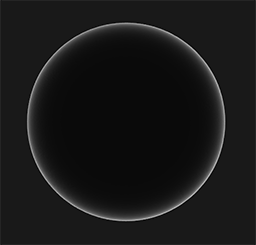
\includegraphics[width=0.4\textwidth]{resources/fresnel}
  \caption{Schlick approximation for a sphere (white is $1$, black is $0$)~\cite{learnopengltheory}}
\label{fig:rayterm-cpu_fresnel}
\end{figure}

Now that the kind of ray has been chosen, the refraction or reflection direction is calculated.
There is an additional possibility that the specific ray we have cannot be refracted because of total internal reflection\,---\,in this case, we switch over to a reflection ray.
The ray direction in the reflection case is calculated with Formula~\ref{Ray Reflection} as in previous materials.
The ray direction in the refraction case is calculated with Formula~\ref{Ray Refraction}.
In this formula, $\eta = \frac{n_{from}}{n_{to}}$ where $n_{from}$ is the index of refraction of the medium we are transfering from and $n_{to}$ is the corresponding index.
Additionally, $I = (\vec{R_{in}} \bullet \vec{S_{normal}})$ where $\vec{R_{in}}$ is the incoming ray and $\vec{S_{normal}}$ is the surface normal.
Finally, $\vec{R_{refract}}$ is the refracted ray.
There is some additional handling in the implementation of this formula to ensure both ray directions (exiting and entering an object) are supported.
This involves flipping the $n$ values and negating $I$ or $\vec{S_{normal}}$.
This formula is derived from the excellent ``Scratchapixel''~\cite{prunier2017shading} and ``Raytracing in One Weekend''~\cite{shirley2016ray}, with some significant rewriting.

\noteworthy{
  \vec{R_{refract}} = \eta\vec{R_{in}} + (\eta I - \sqrt{1 - \eta^2 \cdot (1 - I^2)})\vec{S_{normal}}
}{Ray Refraction}

\subsubsection{Outcome}
\label{ch:methods:renderer:sequential:outcome}

The sequential renderer is only a research prototype and was never finished.
This is primarily because more performance was needed for the final \name{} implementation; the parallel renderer fulfills that need.
Because of the prototype nature of \texttt{rayterm-cpu}, the final implementation only renders images through a Google Test~\cite{googletest} case, which can be run with the \texttt{test.sh} script in the implementation repository~\cite{raytermCpuImpl}, or with \texttt{gradle test}.
This generates a \texttt{test\_image.ppm} file, examples of which we show from various stages of development in Section~\ref{ch:implementation:prototype:raytrace}.
Because of this, \texttt{rayterm-cpu} is very much a proof-of-concept and learning example, rather than a fully-fledged library.

That is not to say that \texttt{rayterm-cpu} was not a useful system.
Many of the algorithms implemented carry over to the parallel renderer, and so the development of that version was aided by existing work.
An excellent example of this is the random generation in \texttt{raymath} and the material scatter functions in \texttt{raytrace}; these algorithms are core to ray-tracing and having a prior implementation simplified further development.
Although they may not carry over unmodified, they are the first iteration in a long improvement cycle.

\subsection{Parallel}
\label{ch:methods:renderer:parallel}

The parallel render engine, \texttt{rayterm-gpu}, uses a Graphics Processing Unit (GPU) to massively parallelize the raytracing algorithm.
This improves performance dramatically because each eye-ray's children (the result of a collision between an object and a ray) are dependant on only their parent eye-ray.
Thus, the computation of a single pixel's color is completely independent of every other pixel.

A short introduction to NVIDIA GPUs may be useful here; they consist primarily of small units of computation circuitry called ``multiprocessors'' which themselves are controllers for several CUDA cores~\cite{fermi2009nvidia}, distributing workloads.
Multiprocessors work on data and code called ``thread blocks.''
Each individual CUDA core in a multiprocessor executes an individual thread in a thread block.
These CUDA cores execute individual threads on the GPU; they can each handle an individual intersection test, and with thousands of them per GPU, we can easily cut the render time down.
There are many restrictions to code that can run in a CUDA thread; CUDA cores act somewhat like advanced floating point arithmetic computation units.
However, OptiX takes care of much of the device handling and thus can perform some advanced optimizations for the individual cores.
A discussion on the specific hardware used for development and testing is available in Section~\ref{ch:intro:background:hardware}.

With 227 commits and over 1.5 thousand lines of code, along with many thousands of additions and deletions, \texttt{rayterm-gpu} has a good start on its life.
There are many, many more improvements possible, however.
We detail some of them in the context of the larger \name{} implementation in Section~\ref{ch:conclusion:future}.
The implementation repository used for \texttt{rayterm-gpu}~\cite{raytermGpuImpl} is also the same used for \name{} as a whole; thus, while we only describe \texttt{rayterm-gpu} in this section, our discussion here also applies to the final \name{} library.
This section specifically covers the \texttt{raytrace} component of the final \name{} library; Section~\ref{ch:methods:interface} covers the \texttt{rayterm} component.
Both of these are combined into a single \texttt{rayterm.so} library for use by other applications.
An example application is also bundled in the implementation repository~\cite{raytermGpuImpl}, as the \texttt{rtexplore} component.
All of these are discussed in more detail in Section~\ref{ch:implementation:final}.

\subsubsection{Libraries}
\label{ch:methods:renderer:parallel:libraries}

Utilizing the massively parallel computation power of a GPU can be difficult\,---\,in fact, before CUDA's release in 2007, there was no well-defined way to do so programmatically.
CUDA is an API and computing platform that enables massively parallel computations~\cite{nvidia2011cuda}.
A special extension of C++, known as CUDA C/C++, can be compiled with \texttt{nvcc}, a custom LLVM-based C/C++ compiler.
This extension enables library support for GPU accelerated multi-threading, physics, and linear algebra, along with many implementations of common data transformation algorithms.
A significant limitation, especially for ray-tracing, is that performance can be significantly affected for inherently divergent tasks\,---\,tasks which do not consistently follow the same control flow\,---\,such as traversing an acceleration structure.

OptiX is an API interface developed for current generation NVIDIA GPUs that enables GPU accelerated ray-object intersection calculations in a programmable pipeline~\cite{parker2010optix, nvidia2019optixdoc}.
It does this by building on top of the CUDA platform, adding abstract and algorithm implementations for common ray-tracing tasks.
OptiX allows user-defined single-ray programs to be compiled into a single program, called a ``kernel,'' that runs on the GPU.
These user programs are written in C++ and then transpiled to PTX, an instruction set for general purpose parallel programming.
Other useful algorithms are also included in the OptiX library, such as BVH and similar acceleration structure implementations.
The main method of communication between host (CPU) and device (GPU) are \texttt{Buffer}s, which are simply arrays managed by OptiX.
Depending on the type of \texttt{Buffer}, data could be moved in one direction or both, depending on the context; an example of this would be the pixel buffer, which is written to on the device and then loaded into CPU-accessible memory for display.

\subsubsection{Programmability}
\label{ch:methods:renderer:parallel:program}

Both OptiX and \name{} itself support programmability in some form.
We will define programmability as the possibility of using user-specified code in some operational capacity at certain points in the program's execution.
For example, it is possible in OptiX to define a CUDA function that will be executed to test if a ray intersects with an object; this enables part of the capability to render any intersectable object with OptiX.
 \name{} supports material programs that are passed on to OptiX to deal with material scatters; because of this it should one day be possible to use NVIDIA MDL materials~\cite{nvidia2015mdl} in \name{}.
We utilize programmability in OptiX in a fairly generic way, because much of the implementation burden for a specific application lies on the application author, and \name{} simply provides an interface.
Before we describe \name{}'s approach, let us consider Figure~\ref{fig:rayterm-gpu_optix_trace}.

\vspace{0.3em}
\begin{figure}[htb]
  \centering
  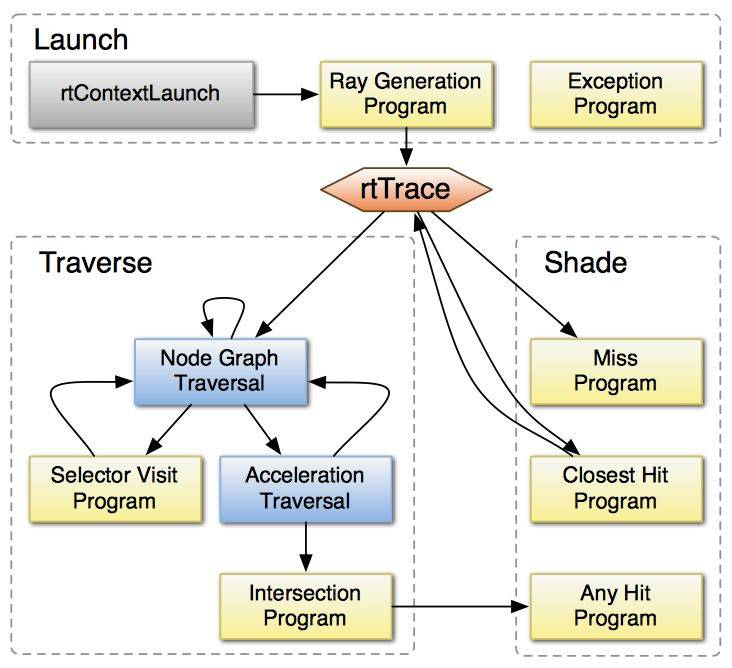
\includegraphics[width=0.7\textwidth]{resources/optix_trace}
  \caption{OptiX Program call graph}
\label{fig:rayterm-gpu_optix_trace}
\end{figure}

In \name{}, we visit only part of Figure~\ref{fig:rayterm-gpu_optix_trace}\,---\,the ``Traverse'' section is not used when RTX mode is enabled: instead, custom intersections and acceleration structures are used for better performance.
In \texttt{rayterm-gpu}, only triangle intersections are supported, and acceleration structure calculations are handed off to OptiX's ``Trbvh'' algorithm~\cite{karras2013fast}.
Triangle intersection and acceleration structure builds are highly optimized in OptiX, more so than any user library could achieve.
In newer NVIDIA RTX GPUs these constraints also enable real hardware acceleration, as opposed to GPU accelerated computation.
In Figure~\ref{fig:rayterm-gpu_optix_trace}, yellow boxes are user-defined programs.
 \name{} defines the Ray Generation Program as a pinhole camera model.
The Exception Program is also defined, with switches to only enable debug prints and exception handling if \name{} is compiled in debug mode.
Lastly, \name{} defines the Miss Program to shade the background of the scene a smooth sky gradient.
The Closest Hit and Any Hit Programs, however, are completely user-defined.
These programs control the scattering of rays when they encounter an object.
How \name{} handles the passthrough configuration of these programs is detailed in the next section.

\name{} supports three asset types: triangle models in the \texttt{OBJ} file format, material definitions in a custom format, and CUDA functions transpiled to PTX, all from arbitrary locations on disk.
These locations are currently specified as compile-time defines \texttt{PROGRAM\_DIRECTORY} and \texttt{ASSET\_DIRECTORY}.
When \name{} or a user application requests a CUDA function, material definition, or object model, these directories are used to search for and load the requested data, which is then inventoried and given an id that the user can reference it with.
This enables easy asset reuse and configurable definition.


\subsubsection{Configurability}
\label{ch:methods:renderer:parallel:config}

At the time of writing, \name{}'s test scene is hard-coded in the \texttt{raytrace} component.
However, it is trivial to provide a loading mechanism so that user applications can specify the scene and any changes to it.
Although the scene itself cannot currently be configured, a wide array of possibilities are available for material and object definitions.
Objects are loaded from an \texttt{OBJ} model file, which should specify at minimum the vertices and vertex normals of the model.
 \name{} uses TinyObjLoader~\cite{tinyobjloader} to load and triangulate \texttt{OBJ} files.
Then, the basic attributes\,---\,vertex positions, normals, shapes, etc.\,---\,are stored in a \texttt{Mesh} object that is inventoried in the resource system.
For materials, a similar process is implemented.
First, a custom parser decodes the given material file, which should conform to the format specified below.
Then, an OptiX \texttt{Material} is created and inventoried.
Finally, the resource system is capable of generating an OptiX \texttt{GeometryInstance}, which links a material and an OptiX \texttt{GeometryTriangles} generated from \texttt{Mesh} data.
This \texttt{GeometryInstance} can then be added to the scene graph and rendered.

\vspace{0.3em}
\begin{figure}[htb]
\centering
\begin{mdframed}[style=MyFrame,nobreak=true,align=center,userdefinedwidth=30em]
\begin{verbatim}
closest:diffuse,closest_hit,0
any:diffuse,any_hit,0
attrib:diffuse,triangle_attributes
var:float3,varAttenuation,0.15,0.86,0.21
\end{verbatim}
\end{mdframed}
\vspace{-0.3em}
\caption{Sample material definition}
\label{fig:rayterm-gpu_material_def}
\end{figure}

In Figure~\ref{fig:rayterm-gpu_material_def} a sample material definition is shown.
The format of a material definition follows a simple pattern: each line is a single ``command,'' the type of which is determined by the element before the first `\texttt{:}'.
There are four types of commands: \texttt{closest}, \texttt{any}, \texttt{attrib}, and \texttt{var}.
The \texttt{closest} command specifies a CUDA function to use for the Closest Hit Program.
It has the format \texttt{closest:<file\_name>,<function\_name>,<ray\_type>}.
The \texttt{any} command is similar, except that it specifies the Any Hit Program.
The \texttt{attrib} command sets the attribute program for the \texttt{GeometryTriangles} instance this material is eventually paired with; it operates on all ray types, and thus does not need a specifier.
Finally, the \texttt{var} command specifies a variable to pass through to the GPU CUDA function; the format is \texttt{var:<type>,<name>,<value>}.
The possible types are \texttt{int} to \texttt{int4}, and \texttt{float} to \texttt{float4}; the values are specified in a comma-separated list.
In Figure~\ref{fig:rayterm-gpu_material_def}, a variable named \texttt{varAttenuation} is defined as $\vec{(0.15,\ 0.86,\ 0.21)}$.
This variable is used in the \texttt{diffuse} PTX file as the color to attenuate the recursively traced ray by\,---\,it is the color of the object this material is applied to.
Any number of commands are allowed, and any later commands will overwrite previous commands if they contain similar information, such as an attrib command.
There is not currently a way to programmatically generate a \texttt{Mesh} or \texttt{Material}, however, these are possible future improvements to \name{}.

% TODO: explain scene description language here (after it is implemented)

\subsubsection{Design}
\label{ch:methods:renderer:parallel:design}

OptiX is heavily utilized in \texttt{rayterm-gpu}.
Much of the \texttt{raytrace} component deals with initializing and configuring the OptiX context correctly.
The main class is \texttt{Renderer}\,---\,it represents a render engine, and has state about the world and everything in it.
\texttt{Renderer} is designed to be a singleton, although no code in \name{} assumes this; rather, each instance requires its own OptiX context.
This could be a problem: according to the OptiX Programming Guide, ``multiple contexts can be active at one time in limited cases, but this is usually unnecessary.''
In that quote, ``limited cases'' really mean that it is untested and not well supported, although technically possible~\cite{nvidia2019optixdoc}.
So depending on future OptiX changes, multi-renderer programs may or may not be a possibility.

A \texttt{Renderer} has three main components that operate on the OptiX context associated with the instance.
The \texttt{Camera} member instance controls the current view of the world and can be used to translate or rotate that view.
The \texttt{Programs} member instance holds an inventory of loaded OptiX CUDA functions and can be used to load more or get existing ones.
Finally, the \texttt{Resources} member instance holds an inventory of \texttt{Material}s and \texttt{Mesh}s; it can also load more or associate existing assets together to produce \texttt{GeometryInstance}s, which could be added to the OptiX scene graph.
There are other smaller supporting classes, such as \texttt{PixelBuffer}, which helps wrap existing OptiX functionality to ensure safe usage.

\subsubsection{Algorithms}
\label{ch:methods:renderer:parallel:algorithms}

The parallel renderer uses many of the same algorithms as \texttt{rayterm-cpu}, so the previous discussion of those still apply.
There are a few new algorithms that are unique to \texttt{rayterm-gpu}, however.
First, a modification of the pinhole camera model was made.
This was inspired by the camera models available in the advanced OptiX samples~\cite{optixsamples}, and simply rewrites the equations used before in terms of $\phi$ and $\theta$, as polar coordinates.
In this new \texttt{Camera}, $\phi$ represents the rotation about the vertical world axis, and $\theta$ the rotation about the horizontal axis.
This enables easier viewing modification so that the look direction can be controlled with just two control axis.
Second, the color output space is transformed into BT.709~\cite{ituBT709}; this ensures color accuracy and gamma correctness, as well as being the assumed color space for \texttt{ppm} files.


\noteworthy{
  L = \left\{
              \begin{array}{ll}
                \frac{V}{4.5} & \quad V < 0.081 \\
                (\frac{V + 0.099}{1.099})^\frac{1}{0.45} & \quad V \geq 0.081
              \end{array}
    \right.
}{BT.709 Conversion}

Formula~\ref{BT.709 Conversion} shows the piecewise function definition for conversion between a raw color value $V$ and a luminance component $L$.
This is done for each color component to get the final color for each pixel.
Additional algorithms also had to be developed as replacements for CPU-based algorithms in CUDA functions.
For example, a \texttt{drand48} implementation is provided for CUDA functions to use, since the existing implementation is CPU-only.
The implementation directly mirrors the UNIX specification for \texttt{drand48}~\cite{drand48UNIX}.
Additionally, the sampling algorithms based off of \texttt{drand48} were replaced with analytical solutions, to prevent sample looping and provide better uniform distribution.
The math behind the analytical solution is based on resources from ``Scratchapixel'' as well as an older paper by the same author as ``Raytracing in One Weekend''~\cite{prunier2017global, shirley1997map}.
We also use an OptiX provided sampler, \texttt{cosine\_sample\_hemisphere}, to generate the initial sample; the further analytical solution simply transforms that sample to the correct normal space.

\noteworthy{
  N_{interpolated} = B_{x} \vec{N_{1}} + B_{y} \vec{N_{2}} + (1 - B_{x} - B_{y}) \vec{N_{0}}
}{Interpolated Normal}

Finally, we use an algorithm to calculate the interpolated shading normal.
This is very loosely derived from the OptiX samples~\cite{optixsamples}, and uses the default \texttt{GeometryTriangles} attribute program to calculate the barycentric coordinates of the intersection point.
Formula~\ref{Interpolated Normal} shows the calculation for obtaining the interpolated normal; this result is normalized and can then be used for reflection or refraction calculations.
An interpolated value is extremely useful because it takes into account the normals of each individual vertex and attempts to ``smooth'' the shape approximated by the triangle, thus making shading more accurate despite the physical differences.
In Formula~\ref{Interpolated Normal}, $N_{i}$ is the vertex normal of the $i$-th vertex in the triangle, and $B$ is the two dimensional barycentric coordinate of the intersection point.
The calculated result, $N_{interpolated}$, is the smoothed normal.
This smoothing can be disabled by using an \texttt{OBJ} model that has had its normals exported as ``flag''\,---\,this causes each triangle's vertices to have their normals all match the face normal, instead of having individual normals.
This is useful for flat faces since the interpolated normal is then simply the same as the face normal.
Figure~\ref{fig:rayterm-gpu_smooth_normal_comparison} shows a comparison between smoothed normals and face normals (sometimes called ``geometric normals'').
Larger versions of these images are available in Appendix~\ref{appendix:large_figures} as Figure~\ref{fig:rayterm-gpu_smooth_normal_comparison_large}

\vspace{0.3em}
\begin{figure}[htb]
  \centering
  \begin{subfigure}[htb]{0.45\textwidth}
    \includegraphics[width=\textwidth]{impl-images/comparisons/before_smooth_normals}
    \caption{Geometric normals (unsmoothed)}
\label{fig:rayterm-gpu_unsmoothed_normals}
  \end{subfigure}
  \hspace{1em}
  \begin{subfigure}[htb]{0.45\textwidth}
    \includegraphics[width=\textwidth]{impl-images/comparisons/after_smooth_normals}
    \caption{Interpolated normals (smoothed)}
\label{fig:rayterm-gpu_smoothed_normals}
  \end{subfigure}
  \caption{Comparison of geometric and interpolated normals}
\label{fig:rayterm-gpu_smooth_normal_comparison}
\end{figure}

\subsubsection{Outcome}
\label{ch:methods:renderer:parallel:outcome}

As part of a larger system and due to reduced available development time, \texttt{rayterm-gpu} has a relatively sparse unit test suite.
Unlike \texttt{rayterm-cpu}, it is tested primarily through integration and comparison tests.
However, \texttt{rayterm-gpu} does meet its goal of increasing performance, so much so that with a GTX 980 Ti GPU, the average render time for a dense scene with tens of thousands of triangles is under 30 milliseconds.
Of course, this is still at a low resolution with only 64 spp; however, this is a vast improvement over the CPU research prototype, which would probably take upwards of an hour on the same scene.
Much of this is due to the massively parallel architecture of OptiX and CUDA.

Just as with \texttt{rayterm-cpu}, a test image can be generated through a Google Test~\cite{googletest} case, which can be run with the \texttt{test.sh} script in the implementation repository~\cite{raytermCpuImpl}, or with \texttt{gradle test}.
This generates a \texttt{test\_image.ppm} file, examples of which we show from various stages of development in Section~\ref{ch:implementation:final:raytrace}.
However, because \texttt{rayterm-gpu} integrates with the larger \name{} system, rendered images can also be seen with the \texttt{rtexplore} sample application, which we discuss in more detail in Section~\ref{ch:methods:interface:sample}.

\section{Terminal Interface}
\label{ch:methods:interface}

The \name{} library depends on two main components: the render engine, and the terminal interface.
This terminal interface uses the render engine to generate images for display in the terminal; it also converts those images from raw pixel colors to unicode characters.
This interface is defined in the actual library, which we discuss in Section~\ref{ch:methods:interface:rayterm}, as well as the user application.
We provide and discuss a sample user application in Section~\ref{ch:methods:interface:sample}.

\subsection{RayTerm}
\label{ch:methods:interface:rayterm}

 \name{} is distinct from \texttt{rayterm}\,---\,\name{} is the entire system, and the name of the project, whereas \texttt{rayterm} is the name of the terminal interface component in the larger implementation.
The interface depends on the \texttt{raytrace} component discussed in Section~\ref{ch:methods:renderer:parallel} to provide a render engine.
Another dependency is \texttt{libtickit}~\cite{libtickitLibrary}, a library that supports ANSI escape code detection and subsequent usage.
Because of the relative obscurity of Tickit, we adapted the main codebase to our needs~\cite{libtickitCustom}; some of these fixes and changes have made their way upstream.

Because of the \texttt{libtickit} usage, \name{} works best in a real XTerm terminal; color output should additionally be enabled by setting the \texttt{COLORTERM} environment variable to \texttt{truecolor}.
These settings are only supported on relatively recent versions of XTerm.
More information of direct color compatibility and the relevant ANSI escape codes can be found in Anton Kochkov's incredibly useful GitHub gist ``TrueColour: Colours in terminal''~\cite{kochkov2019colours}.

\subsubsection{Design}
\label{ch:methods:interface:tickit:design}

There are two important structures in \texttt{rayterm}: the \texttt{UnicodeBuffer} and the \texttt{Terminal}.
The \texttt{UnicodeBuffer} class is a direct analog to \texttt{PixelBuffer},
and can be translated from a \texttt{PixelBuffer} with the \texttt{translate\_halfpixel} function, as we discuss in Section~\ref{ch:methods:interface:tickit:algorithms}.
The \texttt{Terminal} class represents an actual terminal application, with the ability to render a frame, set the information string, resize the terminal, etc.
The \texttt{rayterm} component is actually extremely simple, with just under three hundred lines of code.
Much of the work is handed off to \texttt{libtickit}, which handles the actual character rendering.
In user applications we suggest using \texttt{libtickit} for event loops and other input/output handling, as integrating a different utility may prove difficult given the dependencies of \name{}.

\subsubsection{Algorithms}
\label{ch:methods:interface:tickit:algorithms}

There is only one real algorithm implemented in \texttt{rayterm}: the character translation algorithm.
This algorithm converts a \texttt{PixelBuffer} from the \texttt{raytrace} component to a \texttt{UnicodeBuffer}.
The algorithm, called \texttt{translate\_halfpixel}, has a straightforward implementation: it simply iterates over the pixels in the \texttt{PixelBuffer} two rows at a time, converting the values to \texttt{unicode\_cell} structs.
This two-row iteration is necessary because each unicode character is actually two pixels; the foreground is the ``upper'' pixel, while the background represents the ``lower'' pixel.
The \texttt{unicode\_cell} struct thus holds both a foreground and background color.

This translation algorithm is used to translate each frame's \texttt{PixelBuffer} before rendering the screen; at the time of writing, since only \texttt{translate\_halfpixel} is supported, all characters drawn to the screen are the unicode upper half block character \texttt{U+2580} (see Figure~\ref{fig:unicode_block_characters} for similar example characters).
This causes the foreground color of a \texttt{unicode\_cell} to apply to the character portion of the character cell, and the background color to apply to the empty portion of that same cell.
Through trial and error, we've found that varying the font size through odd values gives the best pixel-like results; even pt sizes can sometimes cause gaps which confuse the viewer.

\subsubsection{Outcome}
\label{ch:methods:interface:tickit:outcome}

While developing the terminal interface was a long and iterative process, the result is a simple and straightforward interface available for use by consumers of the \name{} library.
As with \texttt{rayterm-gpu}, due to time constraints \texttt{rayterm} has a sparse unit test suite; however, its simplicity and reliance on \texttt{libtickit} (which is extremely well tested) lowers the importance of such testing.
For usage, user applications should at minimum simply allocate a new \texttt{Terminal} with the \texttt{new} keyword.
Then, the Tickit \texttt{run} or \texttt{tick} routines should be called to handle re-exposure; otherwise, the terminal will not receive render updates.
A new frame can be drawn (perhaps after modification of the scene graph or camera through the \texttt{Renderer} available in \texttt{Terminal}) with the \texttt{renderFrame} member function.
With this extremely simple interface, complex applications can be designed.


\subsection{RTExplore Sample}
\label{ch:methods:interface:sample}

Within the \name{} implementation repository~\cite{raytermGpuImpl} we provide \texttt{rtexplore}, a simple terminal-based real-time ray-traced viewport into the test world of \texttt{raytrace}.
This sample acts as both an integration test and proof of concept for other users of \name{}.
When running this sample, or indeed any \name{} consumer application, five shared libraries must be linkable; these are listed below.
Depending on how \texttt{libtickit} was compiled into \name{}, \texttt{libtickit.so} may also need to be available.
A video demonstration of \texttt{rtexplore} is available as well~\cite{raytermDemo}.

\vspace{-0.5em}
\begin{itemize}
  \vspace{-0.5em}
  \item \texttt{libtermkey.so}
  \vspace{-0.5em}
  \item \texttt{libunibilium.so}
  \vspace{-0.5em}
  \item \texttt{libcudart.so}
  \vspace{-0.5em}
  \item \texttt{liboptix.so}
  \vspace{-0.5em}
  \item \texttt{librayterm.so}
  \vspace{-0.5em}
\end{itemize}
\vspace{-0.5em}

The \texttt{rtexplore} sample uses a custom Tickit event loop to control input/output, as well as key and mouse event listeners.
The key listener detects key presses in the terminal from the user, and modifies the \texttt{Camera} used for rendering by small amounts;
The A, W, S, and D keys control camera position, while the arrow keys control orientation.
The mouse listener is not used for input, but the caught events are still displayed in the info string, as are past key events.
Thus, most major features of \name{} are utilized by \texttt{rtexplore}.
Of course, this application has huge room for improvement, as does the rest of \name{}.
Some options for future work are provided in Section~\ref{ch:conclusion:future}.


%ch:verify
%
% $Id: ch04_implementation.tex
%
%   *******************************************************************
%   * SEE THE MAIN FILE "AllegThesis.tex" FOR MORE INFORMATION.       *
%   *******************************************************************
%
\chapter{Implementation}\label{ch:implementation}

\section{CPU Prototype}\label{ch:implementation:prototype}

\subsection{\texttt{raymath}}\label{ch:implementation:prototype:raymath}

\subsection{\texttt{raytrace}}\label{ch:implementation:prototype:raytrace}

\section{Final Implementation}\label{ch:implementation:final}

\subsection{\texttt{raytrace}}\label{ch:implementation:final:raytrace}

\subsection{\texttt{rayterm}}\label{ch:implementation:final:rayterm}

\subsection{\texttt{rtexplore}}\label{ch:implementation:final:rtexplore}

\section{Challenges}

CPU:
\begin{enumerate}
  \item metal bug
  \item blender comparisons
  \item space differential
  \item coordinate systems
  \item research difficulty (can't read a physics textbook for each material)
\end{enumerate}

GPU:
\begin{enumerate}
  \item Travis testing
  \item library management
  \item gradle integration
  \item [...]
\end{enumerate}


%ch:conclusion
%
% $Id: conclusion.tex
%
%   *******************************************************************
%   * SEE THE MAIN FILE "AllegThesis.tex" FOR MORE INFORMATION.       *
%   *******************************************************************
%

\chapter{Discussion and Future Work}\label{ch:conclusion}

\section{Summary of Results}\label{ch:conclusion:summary}

\section{Future Work}\label{ch:conclusion:future}

\begin{enumerate}
  \item more materials / MDL support
  \item scene description language
  \item better rtexplore movement
  \item environment image mapping (missed rays => image lookup)
  \item much more...
\end{enumerate}

\section{Conclusion}\label{ch:conclusion:end}

\name\ is a complex system, the implementation and design of which is an ongoing process.
The system currently supports real-time 3D scene viewing through a terminal emulator.
This is made possible through the OptiX library allowing ray-surface intersection calculations to be done a highly parallelized manner on a GPU.
The Tickit interface and its half-pixel translation algorithm, along with \texttt{libtickit} itself, enable \name\ to treat a terminal as an image canvas.
\name\ is now a fully real-time capable ray-tracing engine, rendering 30 or more unicode character images per second to a terminal window on a moderately powerful computer.
Since the initial startup development of \name\ is complete, all contributions to \name\ development are now welcome.
In pursuit of maintaining good open-source readability and ease of development, documentation has been and will continue to be a priority throughout the transition process.
We hope that future projects find \name\ inspiring and useful, whether as an engine or as a jumping-off point for real-time ray-tracing and terminal-based games.

%   ********************************************************************
%   * IF YOU HAVE ANY APPENDICES (FOR INSTANCE, CODE, DATA, GRAPHS,    *
%   * OR ANYTHING ELSE THAT DOESN'T "FIT" AS REGULAR CHAPTER CONTENT), *
%   * INCLUDE THE FOLLOWING LINE, WHICH INSTRUCTS LATEX TO CHANGE FROM *
%   * NUMBERED "CHAPTER" HEADINGS TO LETTERED "APPENDIX" HEADINGS.     *
%   *                                                                  *
%   * APPENDICES HAVE THE SAME FORMATTING COMMANDS AS CHAPTERS (E.G.,  *
%   * "\chapter{...}", "\section{...}", ETC.)                          *
%   ********************************************************************

\appendix

%
% $Id: appa--code
%
%   *******************************************************************
%   * SEE THE MAIN FILE "AllegThesis.tex" FOR MORE INFORMATION.       *
%   *******************************************************************

\chapter{Code}\label{appendix:code}
This appendix lists some miscellaneous code snippets.
However, the main body of work for \name{} is located in two GitHub repsitories, listed in the bibliography as~\cite{raytermCpuImpl} and~\cite{raytermGpuImpl}.


\section{Time Multiplication Operations}\label{appendix:timemul}
\lstinputlisting[language=C++]{code/timemul.cpp}

\chapter{Larger Figures}\label{appendix:large_figures}
This appendix shows larger images for some figures.

\vspace{0.3em}
\begin{figure}[htb]
  \centering
  \includegraphics[width=\textwidth]{impl-images/gpu/hq_complete_1024spp_23s}
  \caption{Final test scene render}
\label{fig:rayterm-gpu_final_render_large}
\end{figure}

\vspace{0.3em}
\begin{figure}[htb]
  \centering
  \begin{subfigure}[htb]{\textwidth}
    \includegraphics[width=\textwidth]{impl-images/comparisons/before_smooth_normals}
    \caption{Geometric normals (unsmoothed)}
\label{fig:rayterm-gpu_unsmoothed_normals_large}
  \end{subfigure}
  \begin{subfigure}[htb]{\textwidth}
    \includegraphics[width=\textwidth]{impl-images/comparisons/after_smooth_normals}
    \caption{Interpolated normals (smoothed)}
\label{fig:rayterm-gpu_smoothed_normals_large}
  \end{subfigure}
  \caption{Comparison of geometric and interpolated normals}
\label{fig:rayterm-gpu_smooth_normal_comparison_large}
\end{figure}

\vspace{0.3em}
\begin{figure}[htb]
  \centering
  \begin{subfigure}[htb]{\textwidth}
    \includegraphics[width=\textwidth]{impl-images/comparisons/before_naive_sampling_change_64spp}
    \caption{Before uniform hemispherical sampling}
\label{fig:rayterm-gpu_hemispherical_sampling_before_large}
  \end{subfigure}
  \begin{subfigure}[htb]{\textwidth}
    \includegraphics[width=\textwidth]{impl-images/comparisons/after_naive_sample_change_64spp}
    \caption{After uniform hemispherical sampling}
\label{fig:rayterm-gpu_hemispherical_sampling_after_large}
  \end{subfigure}
  \caption{Uniform hemispherical sampling}
\label{fig:rayterm-gpu_hemispherical_sampling_large}
\end{figure}

%   *******************************************************************
%   * SEE THE MAIN FILE "AllegThesis.tex" FOR THE "\lstset" COMMAND   *
%   * THAT DEFINES HOW PROGRAM LISTINGS WILL LOOK.                    *
%   *******************************************************************
  % Appendices go here

% only five or six sources uncited, used as auxillary reading basically
% \nocite{*}

\pagebreak

\bibliographystyle{plain}
\bibliography{thesis}
\end{document}
